% \iffalse meta-comment
%
% Copyright (C) 2013-2019 by Walter Daems <walter.daems@uantwerpen.be>
%
% This work may be distributed and/or modified under the conditions of
% the LaTeX Project Public License, either version 1.3 of this license
% or (at your option) any later version.  The latest version of this
% license is in:
% 
%    http://www.latex-project.org/lppl.txt
% 
% and version 1.3 or later is part of all distributions of LaTeX
% version 2005/12/01 or later.
%
% This work has the LPPL maintenance status `maintained'.
% 
% The Current Maintainer of this work is Walter Daems.
%
% This work consists of the files listed in the file manifest.txt.
%
% \fi
%
% \iffalse
%<*driver>
\ProvidesFile{uantwerpendocs.dtx}
%</driver>
%<ct|bmt|mt|le|ex>\NeedsTeXFormat{LaTeX2e}[1999/12/01]
%<ct>\ProvidesClass{uantwerpencoursetext}
%<mt>\ProvidesClass{uantwerpenmasterthesis}
%<bmt>\ProvidesClass{uantwerpenbamathesis}
%<pt>\ProvidesClass{uantwerpenphdthesis}
%<le>\ProvidesClass{uantwerpenletter}
%<ex>\ProvidesClass{uantwerpenexam}
%<ct|bmt|mt|pt|le|ex>    [2019/04/10 v2.4 .dtx skeleton file]
%
%<mt>\errmessage{This class is obsolete, use the uantwerpenbamathesis class instead !}
\def\fileversion{2.4}
\def\filedate{2019/04/10}
%<*driver>
\documentclass{ltxdoc}
\usepackage{makeidx}
\usepackage{alltt}
\usepackage{booktabs}
\usepackage{metalogo}
\IfFileExists{tocbibind.sty}{\usepackage{tocbibind}}{}
\IfFileExists{hyperref.sty}{\usepackage[bookmarksopen]{hyperref}}{}
\EnableCrossrefs
\CodelineIndex
\RecordChanges
\begin{document}
  \DocInput{uantwerpendocs.dtx}
\end{document}
%</driver>
% \fi
%
% \CheckSum{0}
%
% \CharacterTable
%  {Upper-case    \A\B\C\D\E\F\G\H\I\J\K\L\M\N\O\P\Q\R\S\T\U\V\W\X\Y\Z
%   Lower-case    \a\b\c\d\e\f\g\h\i\j\k\l\m\n\o\p\q\r\s\t\u\v\w\x\y\z
%   Digits        \0\1\2\3\4\5\6\7\8\9
%   Exclamation   \!     Double quote  \"     Hash (number) \#
%   Dollar        \$     Percent       \%     Ampersand     \&
%   Acute accent  \'     Left paren    \(     Right paren   \)
%   Asterisk      \*     Plus          \+     Comma         \,
%   Minus         \-     Point         \.     Solidus       \/
%   Colon         \:     Semicolon     \;     Less than     \<
%   Equals        \=     Greater than  \>     Question mark \?
%   Commercial at \@     Left bracket  \[     Backslash     \\
%   Right bracket \]     Circumflex    \^     Underscore    \_
%   Grave accent  \`     Left brace    \{     Vertical bar  \|
%   Right brace   \}     Tilde         \~}
%
%
% \changes{v1.0}{2013/05/11}{\@ Consolidated uacoursetext class and
% uamasterthesis class}
% \changes{v1.1}{2013/05/29}{\@ Small bugfixes and 'filled' option}
% \changes{v1.2}{2014/08/22}{\@ Added lmodern package and increased
% headheight to 13.7pt to please Fancyhdr}
% \changes{v1.3}{2015/12/31}{\@ Minor bugfixes, abondonment of a few
% packages, font freedom}
% \changes{v1.4}{2016/01/07}{\@ Implemented uantwerpenletter class}
% \changes{v1.5}{2016/01/11}{\@ Replaced bottom arcs in footer of
% letter by official PDF versions}
% \changes{v1.6}{2016/02/04}{\@ Added diploma codes for Faculty of
% Applied Economics}
% \changes{v1.7}{2016/05/01}{\@ Added babel translations of elements
% of master's thesis title page}
% \changes{v1.8}{2017/01/08}{\@ Corrected minor typographic mistakes,
% added signature and solved problems with shell escape}
% \changes{v1.81}{2017/01/08}{\@ Bugfixes for release v1.8}
% \changes{v1.9}{2018/03/02}{\@ Integrated uantwerpenexam class into
% package} 
% \changes{v2.0}{2018/05/16}{\@ Implemented uantwerpenphdthesis class
% into package} 
% \changes{v2.1}{2018/06/20}{\@ Bugfix release after promotion event
% on research day}
% \changes{v2.2}{2018/10/23}{\@ Improved visibility of chapter numbers
% by adding a white outline}
% \changes{v2.3}{2019/03/27}{\@ Reworked masterthesis to bamathesis and minor bug fixes}
% \changes{v2.4}{2019/04/10}{\@ Added option for diploma without specialization for EM}
%
%
% \DoNotIndex{\newcommand,\newenvironment}
% \setlength{\parindent}{0em}
% \addtolength{\parskip}{0.5\baselineskip}
%
% \title{The |uantwerpendocs| classes\thanks{This document
% corresponds to \texttt{uantwerpendocs}~\fileversion, dated
% \filedate.}~\thanks{Thanks to Paul Levrie for testing and proofreading.}}
% \author{Walter Daems (|walter.daems@uantwerpen.be|)} 
% \date{\filedate}
%
% \maketitle
%
% \section{Introduction}
%
% This package implements the house style of Universiteit Antwerpen
% for letters, course texts and master/PhD theses. It also implements a
% class to format exams (which is for efficiency reasons and ease of
% copying not fully UAntwerpen house style compliant).
% Using these class files will make it easy for you to make and keep
% your course texts and theses compliant to this version and future
% versions of the UAntwerpen house style. 
%
% If you think (1) there's an error in compliancy w.r.t. the house
% style, (2) there's a feature missing in this class file, or
% (3)there's a bug in this class file, 
% please, contact me through e-mail (|walter.daems@uantwerpen.be|)
% about the issue.
% I'll provide you with an answer and if (and as soon as) possible
% with a solution to the problem you spotted.
%
% Do you like these class files? You're welcome to send us beer, wine,
% or just kind words.
%
% \section{Synopsis}
% The |coursetext|, |bamathesis| and |phdthesis|
% classes\footnote{For readability the class names have been
% abbreviated by omitting the |uantwerpen| prefix} are 
% an extension of the standard \LaTeX{} |book| class.  They are
% intended to be used for writing course texts and master's or PhD
% theses. They provides a title page that is compliant to the
% UAntwerpen house style, and they also typeset the rest of your
% document appropriately. 
%
% The |letter| class is derived from the standard \LaTeX{}
% |letter| class. It is intended to be used for writing business
% letters. It is compliant to the house style and allows for using
% windowed envelopes of the DL format, with right-aligned window.
%
% The |exam| class is derived from the standard \LaTeX{}
% |article| class and is for efficiency reasons not fully UAntwerpen
% house style compliant.
%
% They require (and use) the following packages:
% \begin{itemize}
% \item teh |atbegshi| package
% \item the |auto-pst-pdf| package
% \item the |background| package
% \item the |color| package
% \item the |eso-pic| package
% \item the |etooblox| package
% \item the |fancyhdr| package
% \item the |geometry| package
% \item the |graphicx| package
% \item the |hyperref| package
% \item the |ifthen| package
% \item the |pst-barcode| package
% \item the |tikz| package
% \item the |ulem| package
% \end{itemize}
% and optionally
% \begin{itemize}
%   \item the |varioref| package.
% \end{itemize}
% So make sure these packages are available to your
% \LaTeX{} compiler.
%
% \section{Portability}
% This class file should be ready to use with all common \LaTeX{}
% compilers (PDF\LaTeX{}, \LaTeX{}, \XeLaTeX{}, \LuaLaTeX{}, \ldots)
% from the major \TeX{}-distributions (TeTeX, TexLive, MikTeX). If you
% experience problems, please inform the author.
%
% \section{Usage}
%
% \subsection{Basic Usage}
%
% Use the templates provided below. Remember to \LaTeX{} your source
% file twice in order to have the title and final page correctly
% aligned.
%
% \subsubsection{\texttt{uantwerpencoursetext} class}
% Use the following harness for your \LaTeX{} course text:
% \begin{verbatim}
% \documentclass[a4paper]{uantwerpencoursetext}
%
% \usepackage{<include any packages you require here>}
%
% \facultyacronym{<put your faculty's acronym here}
%
% \title{<put your title here>}
% \subtitle{<put your subtitle here>}
% \author{<put your name here>}
%
% \courseversion{<put a version identifier here>}
% \versionyear{<the publication date of the course here>}
% 
% \lecturer{<person teaching the course>}
% \programme{<descriptor of first programme>}
% \course{<course code>}{<name of the course>}% 
%
% \academicyear{<XXXX-YYYY>}
%
% \begin{document}
%
%   \maketitle
%
%   % put your LaTeX code here
%
%   \finalpage
%
% \end{document}
% \end{verbatim}
%
% The available faculty acronyms are listed in a table on page
% \pageref{acronyms}. 
%
% \subsubsection{\texttt{uantwerpenbamathesis} class}
% Use the following harness for your \LaTeX{} bachelor or master's
% thesis: 
% \begin{verbatim}
% \documentclass[a4paper]{uantwerpenbamathesis}
%
% \usepackage{<include any packages you require here>}
%
% \facultyacronym{<put your faculty's acronym here>}
%
% \title{<put your title here>}
% \author{<put your name here>}
% \supervisori{<put supervisor's name(s) here>}{<affiliation goes here>}
% \supervisorii{<put supervisor's name(s) here>}{<affiliation goes here>}
% \supervisoriii{<put supervisor's name(s) here>}{<affiliation goes here>}
% \supervisoriv{<put supervisor's name(s) here>}{<affiliation goes here>}
%
% % classmarker
% \academicyear{<XXXX-YYYY>}
%
% \begin{document}
%
%   \maketitle
%
%   % put your LaTeX code here
%
%   \finalpage
%
% \end{document}
% \end{verbatim}
%
% The available faculty acronyms are listed in a table on page
% \pageref{acronyms}. 
% 
% \subsubsection{\texttt{uantwerpenletter} class}
% Use the following harness for your \LaTeX{} letter:
% \begin{verbatim}
% \documentclass[a4paper]{uantwerpenletter}
%
% % setup fonts according to your specific TeX compiler setup
%
% \usepackage{<include any packages you require here>}
%
% % \logo{} only specify if you want to use your unit's logo
%
% \sender{<put your name here>}{<put your title/role here>}
% \facultyacronym{<put your faculty's acronym here>}
% \unit{<put your unit here>}
% \address{<put your multi-line address here>}
% \email{<user name>}{<domain name>}
% \phone{<put your phone number here, start with +32>}
% \fax{<put your fax number here, start with +32>}
% \mobile{<put your mobile number here, start with +32>}
% \returnaddress{<put your single-line return address here>}
%
% \to{<name of the addressee goes here>}
% \toorganization{<name of the organization goes here>}
% \toaddress{<multi-line address of the addressee goes here>}
% 
% \date{<specify date - otherwise today>}
% \subject{<specify subject>}
%
% \begin{document}
%
%   \maketitle % generates top of the letter
%
%   \opening{Dear <name>}
% 
%   <write your letter here>
%
%   \closing{Kind regards,}
%
%   \carboncopy{<put CC people here>}
%   \enclosed{<put reference to enclosed documents here>}
%
% \end{document}
% \end{verbatim}
%
% The available faculty acronyms are listed in a table on page
% \pageref{acronyms}. You may use lists in the |\carboncopy| and
% |\enclosed| commands. The spacing will be compact.
%
% \subsubsection{\texttt{uantwerpenphdthesis} class}
%
% \begin{verbatim}
% \documentclass[b5paper,10pt,twoside,openright,filled]{uantwerpenphdthesis}
%
% You may want to use common fonts
% \usepackage{<include any additional packages you require here>}
% 
% \title{<put your title here>}
% \author{<put your name here>}
% \facultyacronym{<put your faculty's acronym here>}
% \programme{PHD}
%           {<put your programme's acronym here>}
%           {<put your specialization's acronym here>}
% \affiliation{<put your affiliation here>}
% \address{<put your contact details here>}
% 
% \supervisori{<put supervisor's name here>}{<affiliation goes here>}
% \supervisorii{<put supervisor's name here>}{<affiliation goes here>}
% 
% \jurychairman{<put chairman's name here>}{<affiliation goes here>}
% 
% \jurymemberi{<put member's name here>}{<affiliation goes here>}
% \jurymemberii{<put member's name here>}{<affiliation goes here>}
% \jurymemberiii{<put member's name here>}{<affiliation goes here>}
% 
% \phddegree{<put official degree name here>}
% \defenselocation{<put location of defense here>}
% \defensedate{<put defense year here>}
% \titlepageimage{<set file name of title page image here>}
% 
% \isbn{<put ISBN13 number here>}
% \depot{<put Depot number here>}
% 
% \begin{document}
% 
% \maketitle
% \frontmatter
% \tableofcontents
% \mainmatter
% 
% % write your PhD text here
% 
% \appendix
% 
% % write appendix material here
% 
% \makefinalpage
% 
% \end{document}
% \end{verbatim}
%
% \subsection{The class options explained}
%
% The classes have several options. They are listed below.
% After every option, it has been indicated to which class the option
% applies (between square brackets, without prefix uantwerpen).
% \changes{v1.1}{2013/05/28}{Added option user documentation}
%
% \DescribeMacro{copyright} [coursetext]\\
%   This option forces printing a watermark on every page. For the
%   paper version of your document, this is inappropriate, but for any
%   e-copy you make available, this may be appropriate;
%
% \DescribeMacro{examiner} [exam]\\
%   This option allows to set the exam class in examiner mode,
%   mentioning the examiner mode on every page (as regular text in the
%   header and also in a watermark) to make sure you never hand out
%   that copy to students and suppressing the fillout pages.
%
% \DescribeMacro{filled} [letter / coursetext /
% bamathesis / phdthesis]\\ 
%   This option causes the text to be filled (simultaneous left and
%   right alignment). Though this setting is not recommended, it is
%   provided because the default |\raggedright| cannot be undone. The
%   |filled| option prevents the |\raggedright| from being
%   issued. However, if you care about the typographic readability of
%   your text, you shouldn't use this option.
%
% \DescribeMacro{titlepagenoartwork} [coursetext /
% bamathesis / phdthesis]\\
%   This option forces the title pages to be typeset without circle graphics and
%   logo. This allows for printing on a pre-printed color sheet that
%   already contains circle graphics and logo;
%
% \DescribeMacro{titlepagetableonly} [coursetext /
% bamathesis / phdthesis]\\ 
%   This option forces the title-page data to be printed in table form
%   as first page. Some publishers require the manuscript to be
%   delivered in this form. They perform the entire typesetting of the
%   title page.
%
% \DescribeMacro{qr} [coursetext]\\
%   This option allows you to generate a QR code containing the details of
%   the course on the title page or the table-only title page. For
%   this option to work, the package pstricks is loaded. It will not
%   work with pdf\LaTeX{} unless you enable shell escape. Read your
%   pdf\LaTeX{}-package documentation on how to do that.
%
% Common sets of options depend on the purpose:
% \begin{itemize}
% \item to make a text ready for electronic distribution:
% |a4paper|, |copyright|.
% \item to make a camera-ready text (for printing) in case
% the cover is printed on a pre-printed color artwork cover sheet is:
% |a4paper|, |qr|, |titlepagenoartwork|.
% \item to make a camera-ready text (for printing) in case the cover
% is typeset based on table data:
% |a4paper|, |qr|, |titlepagetableonly|. 
% \item to make a letter:
%   no options (filling a letter is discouraged)
% \item to make an exam:
%   no options (filling an exam is discouraged)
% \item to make a PhD text:
%   |b5paper|, |twoside|, |openright| and |filled|
% \end{itemize}
%
% \subsection{The macros explained}
%
% \subsubsection{Common macros}
%
% After every macro, it has been indicated to which class the macro
% applies (between square brackets), and whether it is mandatory or not.
%
% \DescribeMacro{\facultyacronym} [coursetext /
% bamathesis / phdthesis / exam] (mandatory)\\
% \label{md-facultyacronym}
% This macro sets the acronym of the faculty.
% This macro also sets the faculty name according to the specified
% acronym.
% If you're missing a faculty or institute, please ask the
% author to complete the list.
% 
% The available acronyms are:
% \changes{v1.9}{2018/03/02}{\@ Added ASoE (Antwerp School of Education)}
% \label{acronyms}
% \begin{center}
% \begin{tabular}{cl}
%   \toprule
%   Acronym & Faculty name \\
%     \midrule
%   ASoE
%   & Antwerp School of Education\\
%   CPG
%   & Centrum Pieter Gillis\\
%   FBD 
%   & Faculteit Farmaceutische, Biomedische en Diergeneeskundige Wetenschappen\\
%   GGW    
%   & Faculteit Geneeskunde en Gezondheidswetenschappen\\
%   IOB
%   & Instituut voor Ontwikkelingsbeleid- en beheer\\
%   IOIW
%   & Instituut voor Onderwijs- en Informatiewetenschappen\\
%   LW
%   & Faculteit Letteren en Wijsbegeerte\\
%   OW
%   & Faculteit Ontwerpwetenschappen\\
%   SW
%   & Faculteit Sociale Wetenschappen\\
%   REC
%   & Faculteit Rechten\\
%   TEW
%   & Faculteit Toegepaste Economische Wetenschappen\\
%   TI     
%   & Faculteit Toegepaste Ingenieurswetenschappen\\
%   WET    
%   & Faculteit Wetenschappen\\
%   \bottomrule
% \end{tabular}
% \end{center}
%
% \subsubsection{Macros for the coursetext, bamathesis, phdthesis
% classes}
%
% \DescribeMacro{\academicyear} [coursetext / bamathesis]
% (mandatory)\\
% Use this macro to specify the academic year in full, i.e. in the
% form |XXXX-YYYY|. 
% 
% \DescribeMacro{\author} [coursetext / bamathesis / phdthesis ] (mandatory)\\ 
% This macro sets the author of the document.
% It also sets the |pdfauthor| tag of the hyperref package, so that
% the PDF-document meta-information is correct.
%
% \DescribeMacro{\copyrightnotices} [coursetext]
% (optional)\\ 
% Use this macro to specify additional copyright notice messages to
% appear in the copyright notice on the bottom of page 2 of your
% course text.
% 
% \DescribeMacro{\course} [coursetext] (mandatory)\\
% \label{dm-course}
% Code (first argument) and name (second argument) of the curriculum
% course this coursematerial or exam belongs to. The code should be of
% the form:\\ 
% |TNNNFFFAAA|,
% with:
% \begin{center}
%   \begin{tabular}{cp{10cm}}
%     \toprule
%       Code & Explanation \\
%     \midrule
%       |T|    & a number indicating the type of programme \\
%              & (1 for Bachelor courses, 2 for Master courses , 5 for
%                specific courses of preparatory programmes) \\
%       |NNN|  & a number assigned by the Faculty's administration\\
%       |FFF|  & the acronym of your Faculty, e.g., FTI\\
%       |AAA|  & an alphanumeric code assigned by the Faculty's
%                administration \\
%     \bottomrule
%   \end{tabular}
% \end{center}
%
% An example of such a code: 1001FTIWIS, for the first-semester
% mathematics course of the Faculty of Applied Engineering.
%
% For courses of the Faculty of Applied Engineering, the name should
% be of the form |x-YYYYYYYY| with |x| the number of the
% semester and |YYYYYYYY| the official name of the course.
%
% In case the course's name contains accented characters, one should
% also provide a qr version, containing utf8-characters only.
% The macro for this purpose takes only one argument, i.e. the
% course's name! This is to avoid inconsistencies in the course codes.
%
% \DescribeMacro{\courseversion} [coursetext] (optional)\\
% This macro indicates which version of the course this is.
%
%
% \DescribeMacro{\defensedate} [bamathesis / phdthesis] (mandatory)\\
% Date of the bamathesis defense in Dutch, in the form 'month year',
% e.g. ``juni 2012''. In case of a PhD thesis, only the year should be
% mentioned. 
% 
% \DescribeMacro{\defenselocation} [bamathesis / phdthesis]
% (optional)\\ 
% Location of the defense. Defaults to ``Antwerpen''.
%
%
% \changes{v1.6}{2016/02/04}{Added diploma code documentation}
% \changes{v2.0}{2018/05/16}{Updated diploma code documentation to
% incorporate PhD degrees}
% \changes{v2.3}{2019/03/27}{Introduced bachelor level codes to allow for bachelor theses}
% \DescribeMacro{\diploma} [bamathesis] (mandatory)\\
% This must be the official title, in Dutch. To avoid errors, we chose
% to use specific codes, that will expand to the correct description.
% These codes are specific for the Faculty of Applied Engineering. If
% you want the author of the package to add codes for your faculty,
% just ask!
% \begin{center}
%   \begin{tabular}{lp{10cm}}
%     \toprule
%     Code & Description (in Dutch!) \\
%     \midrule
%       \multicolumn{2}{c}{Faculteit Toegepaste
%       Ingenieurswetenschappen}\\ 
%     \midrule
%     \midrule
%     |BA-IW-BK| 
%     & Bachelor of Science in de industri\"ele wetenschappen: bouwkunde\\
%     |BA-IW-BCH| 
%     & Bachelor of Science in de industri\"ele wetenschappen: biochemie\\
%     |BA-IW-CH|
%     & Bachelor of Science in de industri\"ele wetenschappen: chemie\\
%     |BA-IW-EI|
%     & Bachelor of Science in de industri\"ele wetenschappen: elektronica-ICT\\
%     |BA-IW-EM|
%     & Bachelor of Science in de industri\"ele wetenschappen: elektromechanica\\
%     |MA-IW-BK| 
%     & Master of Science in de industri\"ele wetenschappen: bouwkunde\\
%     |MA-IW-BCH| 
%     & Master of Science in de industri\"ele wetenschappen: biochemie\\
%     |MA-IW-CH|
%     & Master of Science in de industri\"ele wetenschappen: chemie\\
%     |MA-IW-EI|
%     & Master of Science in de industri\"ele wetenschappen: elektronica-ICT\\
%     |MA-IW-EI-AE|
%     & Master of Science in de industri\"ele wetenschappen: elektronica-ICT,
%     afstudeerrichting, Automotive Engineering\\
%     |MA-IW-EI-ICT|
%     & Master of Science in de industri\"ele wetenschappen: elektronica-ICT,
%     afstudeerrichting ICT\\
%     |MA-IW-EM|
%     & Master of Science in de industri\"ele wetenschappen: elektromechanica\\
%     |MA-IW-EM-AE|
%     & Master of Science in de industri\"ele wetenschappen: elektromechanica,
%     afstudeerrichting Automotive Engineering\\
%     |MA-IW-EM-AU|
%     & Master of Science in de industri\"ele wetenschappen: elektromechanica,
%     afstudeerrichting Automatisering\\
%     |MA-IW-EM-EM|
%     & Master of Science in de industri\"ele wetenschappen: elektromechanica,
%     afstudeerrichting Elektromechanica\\
%     |MA-IW-EM-EN|
%     & Master of Science in de industri\"ele wetenschappen: elektromechanica,
%         afstudeerrichting Energie\\
%     |PHD-TI-BK|
%     & Doctor in de Toegepaste Ingenieurwetenschappen: bouwkunde\\
%     |PHD-TI-BCH|
%     & Doctor in de Toegepaste Ingenieurwetenschappen: biochemie\\
%     |PHD-TI-CH|
%     & Doctor in de Toegepaste Ingenieurwetenschappen: chemie\\
%     |PHD-TI-EI|
%     & Doctor in de Toegepaste Ingenieurwetenschappen: elektronica-ICT\\
%     |PHD-TI-EM|
%     & Doctor in de Toegepaste Ingenieurwetenschappen: elektromechanica\\
%     \midrule
%       \multicolumn{2}{c}{Faculteit Toegepaste Economische
%       Wetenschappen}\\
%     \midrule
%     |MA-TEW-HI| 
%     & Master of Science in de toegepaste economische wetenschappen:
%     handelsingenieur\\
%     |MA-TEW-HIBI| 
%     & Master of Science in de toegepaste economische wetenschappen:
%     handelsingenieur in de beleidsinformatica\\
%     |MA-TEW-EB|
%     & Master of Science in de toegepaste economische wetenschappen:
%     economische beleid\\
%     |MA-TEW-BK|
%     & Master of Science in de toegepaste economische wetenschappen:
%     bedrijfskunde\\
%     \bottomrule
%   \end{tabular}
% \end{center}
%
% \DescribeMacro{\lecturer} [coursetext] (mandatory)\\
% This is the name of the person that actually teaches the course (in
% Dutch: titularis). If there are multiple persons, please, use the
% macros |\lectureri|, |\lecturerii|, |\lectureriii|,
% |\lectureriv|. 
%
% \DescribeMacro{\phddegree} [phdthesis] (mandatory)\\
% This is the official degree name (in the appropriate language,
% possibly mixed ``dutch (english)'').
%
% \DescribeMacro{\programme} [coursetext] (mandatory)\\
% \label{dm-programme}
% This macro takes three arguments (for the time being, only
% applicable to the faculty of applied engineering):
% \begin{itemize}
% \item the type of the programme: BA, SP, VP or MA
% \item the domain of the programme: IW
% \item the qualifier of the programme: BK, CH, BCH, EM, EI
% \end{itemize}
% If you need more programme classes or qualifiers, ask the author to
% complete the available codes.
% Correct usage of the macro will result in error-free descriptions on
% your title page.
% You can overrule the standard descriptions, by specifying 'FREE' as
% first argument and a free text description as second, leaving the third
% one empty. However, we strongly advise against taking this route.
% Instead, ask the author to complete the available codes.
%
% \DescribeMacro{\publisher} [coursetext] (mandatory)\\
% This macro sets the publisher information of the document.
% It is printed on the front page. It defaults to the repographic
% service of campus Groenenborger, one of the standard printing
% services of Universiteit Antwerpen.
%
% \DescribeMacro{\publishercode} [coursetext] (mandatory)\\
% This macro sets the publisher code of the document.
% It is printed on the front page. This is code that the publisher
% uses for its internal administration. It may be a proprietary code,
% or an ISBN number.
%
% \DescribeMacro{\subtitle} [coursetext / phdthesis] (optional)\\
% This macro sets the title of the document. You may use this 
% \begin{itemize}
% \item to further clarify the title
% \item to indicate the nature of this document
% \end{itemize}
% The latter is to be considered when you want to provide multiple
% documents as parts of the full course text (e.g., Course Notes,
% Formula Collection, Exercise Book, Solution Book).
% This macro also sets the |subject| tag of the hyperref package,
% so that the PDF-document meta-information is correct.
%
% \DescribeMacro{\supervisor} [bamathesis / phdthesis] (mandatory)\\
% This is the name of the person that promotes/supervises the thesis.
% Please, use the macros |\supervisori|, |\supervisorii|, |\supervisoriii|,
% |\supervisoriv|. 
%
% \DescribeMacro{\title} [coursetext / bamathesis / phdthesis] (mandatory)\\ 
% This macro sets the title of the document.
% It also sets the |pdftitle| tag of the hyperref package, so that
% the PDF-document meta-information is correct.
%
% \DescribeMacro{\titlepageimage} [phdthesis]
% (optional)\\
% This sets the central image on the title page to appear clipped
% within the curves.
%
% \DescribeMacro{\versionyear} [coursetext] (mandatory)\\
% This is to be the year in which you published the current version of
% the course in the form YYYY.
%
% 
% \subsubsection{Macros for the letter class}
%
% \DescribeMacro{\address} [letter] (mandatory)\\
% Address of the sending unit (or faculty). This can be different from
% the return address. Newlines are allowed and encouraged.
%
% \DescribeMacro{\carboncopy} [letter] (optional)\\
% List of persons receiving a copy of this letter. Format at will.
%
% \DescribeMacro{\closing}  [letter] (mandatory) \\
% Closing clause of the letter. E.g. 'Best regards,'.
%
% \DescribeMacro{\date} [letter] (optional) \\
% Date of the letter. If not specified today's date (at the time of
% running \LaTeX{}) will be used.
%
% \DescribeMacro{\email} [letter] (optional)\\
% E-mail address of the sending person, or the administrative person
% tracking the letter. This must definitely be someone that can answer
% questions related to this letter.
% \begin{itemize}
% \item first argument: user name
% \item second argument: domain name
% \end{itemize}
%
% \DescribeMacro{\enclosed} [letter] (optional)\\
% List of enclosed documents. Format at will.
%
% \DescribeMacro{\fax} [letter] (optional)\\
% Probably facsimile is not used anymore, but anyway: fax number of
% the sending person. See also |\email|.
%
% \DescribeMacro{\logo} [letter] (optional)\\
% file name of an alternative logo to use. The file name must be the
% name of a file in the search path of type PDF.
% If this macro is not used, The default logo of the university will
% be used.
%
% \DescribeMacro{\mobile} [letter] (optional)\\
% Mobile phone number of the sending person. See also |\email|.
%
% \DescribeMacro{\opening}  [letter] (mandatory) \\
% Opening address of the letter. E.g. 'Dear X,'.
%
% \DescribeMacro{\phone} [letter] (optional)\\
% Phone number of the sending person. See also |\email|.
%
% \DescribeMacro{\returnaddress} [letter] (mandatory)\\
% This is a short return address (listed in small font on top of the
% destination address (such that it is visible in a windowed envelope
% (European format)). It should fit on a single line. Typically we list
% an acronym for the unit, a room number, a campus name and address.
% The goal is to get the undelivered letter back to the person that
% can take action accordingly.
%
% \DescribeMacro{\sender} [letter] (mandatory)\\
% Description of the person writing the letter.
% \begin{itemize}
% \item first argument: name of the person writing the letter
% \item second argument: title / role of the person
% \end{itemize}
% Newlines are not allowed in the arguments.
%
% \DescribeMacro{\signature}  [letter] (optional) \\
% Add a signature (in between the closing statement of the
% letter and the sender's name. This might be a text message or a
% picture of your signature.
%
% \DescribeMacro{\subject} [letter] (mandatory) \\
% Short descriptive subject that describes the contents of the
% letter.
%
% \DescribeMacro{\to} [letter] (mandatory)\\
% Name of the addressee. Newlines are allowed. 
% Preferably name and role are split over two lines.
%
% \DescribeMacro{\toaddress} [letter] (mandatory)\\
% Address of the addressee. Newlines are allowed. The address should
% fit on max. 3 lines.
%
% \DescribeMacro{\toorganization} [letter] (optional)\\
% Name of the organization that employs the addressee.
%
% \DescribeMacro{\unit} [letter] (optional)\\
% Name of the unit to which the person belongs. This can be a
% research group, a laboratory, an administrative division, etc.
% Newlines are allowed.
%
% \subsubsection{Macros for the exam class}
%
% \DescribeMacro{\author} [exam] (mandatory)\\
% The author of the exam (may be multiple authors, separated by
% commas). On the title page, these will be labeled as 'Professor(s) -
% Titularis(sen)'.
%
% \DescribeMacro{\academicyear} [exam] (mandatory)\\
% Use this macro to specify the academic year in full, i.e. in the
% form |XXXX-YYYY|.
%
% \DescribeMacro{\course} [exam] (mandatory)\\
% see description of |\course| macro on page~\pageref{dm-course}.
%
% \DescribeMacro{\examdate}
% specifies the date of the exam. We recommend the YYYY-MM-DD format,
% but you are free to chose your own coding scheme for dates. We
% advize against using UNIX epoch time, to avoid problems in the first
% semester exams in 2038.
%
% \DescribeMacro{\examgroupnumber} [exam]\\
% mentions the group number (may be empty)
%
% \DescribeMacro{\examlength}
% specifies the length of the exam in a unit of time, e.g. '4h'
%
% \DescribeMacro{\exampart} [exam] (mandatory)\\
% Description of the part of the course the exam covers.
% Often the evaluation of a course consists of multiple evaluation
% elements (e.g. a written exam, a portfolio defense and lab
% reports). Using this macro you can indicate the part this exam
% covers. E.g. it could be 'Written Exam' (to distinguish from the
% other parts 'portfolio defense' and 'lab reports').
%
% \DescribeMacro{\extrainfo}
% specifies the extra information that appears on the back of the
% title page, regarding the materials that can be used during the
% examination and cautioning the students not to commit fraude.
% You can specify an optional first argument 'firstpage', such that
% your extra info starts on the first page, below the title block. In
% that case the extra info will also not be terminated with a
% clearpage (as we assume you want to conserve space).
%
% \DescribeMacro{\programme} [exam] (mandatory)\\
% see description of |\programme| macro on page~\pageref{dm-programme}.
%
% \DescribeMacro{\rooms}
% specifies the rooms in which the exam will take place. This is
% useless info for the student, but may be of convenience for you as
% author or supervisor of the exam. Use UAntwerpen standard room
% designators, e.g. 'G.U.025' for room number 025, on the
% Groenenborgercampus in the U-building.
%
% \DescribeMacro{\studentnr}
% specifies the exam copy number. This will appear on every page of
% the exam, easing the reassembly of pages that do not contain any
% name. Moreover, it allows for blind correction as the student only
% writes his name ot he front page.
%
% \DescribeMacro{\tend}
% specifies the end time of the exam in a format identical to the one
% chosen for |\tstart|.
%
% \DescribeMacro{\tstart}
% specifies the start time of the exam, preferrable in the format
% 'HHhMM', e.g. '08h30'.
%
% \subsection{Examples}
% \subsubsection{\texttt{uantwerpencoursetext}}
%
% This example uses the |qr| option (that invokes the |auto-pst-pdf|
% package) so enable 'write18' or 'shell-escape' for your \LaTeX{}
% compiler.
%
% \begin{verbatim}
%<*ct-example> 
\documentclass[a4paper,11pt,oneside,openright,english,qr,copyright]{uantwerpencoursetext}

\usepackage[english,dutch]{babel}
\usepackage{lipsum}  % this is just for some dummy text, please remove

\title{Z\'agen, zoeken en zuchten}
\qrtitle{Zágen, zoeken en zuchten}
\subtitle{Cursusnota's}
\author{Walter Daems en Paul Levrie}

\courseversion{1.3}
\versionyear{2016}

\lectureri{Zoltan Zo\"ekers}
\qrlectureri{Zoltan Zoëkers}
\lecturerii{Siana Sigh}
\lectureriii{Zeger de Z\'ager}
\qrlectureriii{Zeger de Záger}

\facultyacronym{TI}
\programme{MA}{IW}{EI}
\coursei{2023FTIZZZ}{5-Zoekmachines in een zaagperspectief}
\courseii{2045FTIIII}{6-Zaagmachines in \'e\'en zuchtperspectief}
\qrcourseii{6-Zaagmachines in één zuchtperspectief}

\academicyear{2015-2016}


\publisher{Universiteit Antwerpen\\
  Cursusdienst en reprografie\\
  Campus Groenenborger, G.U.027\\
  Groenenborgerlaan 171\\
  2020 Antwerpen\\
  T +32 3 265 32 15\\
  F + 32 3 233 32 27\\
  E cursusdienst.cgb@uantwerpen.be}

\publishercode{C11111102}

\copyrightnotices{
  The graphics in this document have been typeset using \texttt{TikZ}.\\
  This document has been \TeX-ed on a GNU/Linux workstation.
}

\begin{document}
\selectlanguage{dutch} % or english if your text is in English

\maketitle

\frontmatter

\tableofcontents

\mainmatter
\chapter*{Inleiding}
\lipsum[1]
\chapter{Onzin voor dummies}

\section{Het gebeuren}
\lipsum[2]
\begin{equation}
  e^{-j\pi} + 1 = 0
\end{equation}

\lipsum[3]
\section{En waartoe het geleid heeft}

\lipsum[4]

\subsection{Herhaling}

\lipsum[5]

\subsection{Begint vervelend te worden}

\lipsum[6]
\newpage

\subsection{Begint echt vervelend te worden}

\lipsum[7-10]

\chapter{Besluit}

\appendix

\chapter{Symbolen}
\chapter{Romeinse sprekers}
\chapter{Referentielijst}

\makefinalpage

\end{document}
%</ct-example> 
% \end{verbatim}
% 
% 
% \subsubsection{\texttt{uantwerpenbamathesis}}
% 
% \begin{verbatim}
%<*bmt-example> 
\documentclass[a4paper,11pt,twoside,openright,english]{uantwerpenbamathesis}

\usepackage[english]{babel} % or dutch if your text is in Dutch
\usepackage{lipsum}  % this is just for some dummy text, please remove

\title{Minimax optimisatie voor performantieruimtemodellering}
\author{Bert Bibber}

\supervisori{Prof. dr. ir. Kumulus}{Universiteit Antwerpen}
\supervisorii{Prof. dr. Hilarius Warwinkel}{TNT-Bang, N.V.}
\supervisoriii{ing. Piet Pienter}{POM}

\facultyacronym{TI}
\academicyear{2015-2016}
\diploma{MA-IW-EM}
\defenselocation{Antwerpen}
\defensedate{juni 2016}

\begin{document}

\maketitle

\frontmatter

\tableofcontents

\mainmatter
\chapter*{Inleiding}

\lipsum[1]

\chapter{Onderzoeksvraag}

\section{Het gebeuren}

\lipsum[2]

\begin{equation}
  e^{-j\pi} + 1 = 0
\end{equation}

\lipsum[3]

\chapter{Literatuurstudie}

\chapter{Theoretische achtergrond}

\chapter{Eigen realisatie}

\chapter{Besluit}

\appendix

\chapter{Symbolen}
\chapter{Referentielijst}

\makefinalpage

\end{document}
%</bmt-example> 
% \end{verbatim}
% 
%
% \subsubsection{\texttt{uantwerpenphdthesis}}
%
% \paragraph{Dutch}
% \begin{verbatim}
%<*pt-example1> 
\documentclass[b5paper,10pt,twoside,openright,filled]{uantwerpenphdthesis}

% You may want to use common fonts
\usepackage{mathptmx}
\usepackage{fontspec}
\setsansfont{Calibri}

\usepackage[dutch]{babel} % or dutch if your text is in Dutch
\usepackage{lipsum}  % this is just for some dummy text, please remove

\title{Harmonische Signaalanalyse\\met behulp van Lineaire
  Operatoren}
\subtitle{Waarom moeten titels van doctoraatsthesissen toch altijd
  lang en onverstaanbaar zijn?}
\author{Ing. Theofiel Hoekaff}
\facultyacronym{TI}
\programme{PHD}{IW}{EI}
\affiliation{Universiteit Antwerpen\\
  Faculteit Toegepaste Ingenieurswetenschappen\\
  Constrained Systems Lab (CoSys-Lab)}
\address{Groenenborgerlaan 171, 2020 Antwerpen, Belgi\"e\\
  M: theofiel.hoekaff@uantwerpen.be\\
  T: +32 265 00 00
}

\supervisori{Prof. dr. W. Vlaams}{Universiteit Antwerpen, Belgi\"e}
\supervisorii{Prof. dr. J. Stekker}{Universiteit Antwerpen, Belgi\"e}

\jurychairman{Prof. dr. P. Dalinckx}{Universiteit Antwerpen, Belgi\"e}

\jurymemberi{Prof. dr. J. Dezerooder}{Universiteit Antwerpen, Belgi\"e}
\jurymemberii{Prof. dr. P. De Tollenaere}{Flanders Make, Belgi\"e}
\jurymemberiii{Prof. dr. M. Byr}{IMEC, Nederland}

\phddegree{doctor in de toegepaste ingenieurswetenschappen}
\defenselocation{Antwerpen}
\defensedate{2018}
\titlepageimage{keyboard.jpg}

\isbn{987-90-57285-34-7}
\depot{D/2018/12.293/03}

\begin{document}

\maketitle

\frontmatter

\tableofcontents

\mainmatter
\chapter*{Inleiding}

\lipsum[1]

\chapter{Onderzoeksvraag}

\section{Het gegeven}

\lipsum[2]

\begin{equation}
  e^{-j\pi} + 1 = 0
\end{equation}

\lipsum[3-17]

\chapter{Literatuurstudie}

\lipsum[18-19]

\chapter{Theoretische achtergrond}

\lipsum[20-21]

\chapter{Eigen realisatie}

\lipsum[22-24]

\chapter{Besluit}

\lipsum[25]

\appendix
\chapter{Symbolen}

\chapter{Publicaties}
% Put your bibliography here using BibTeX

\makefinalpage

\end{document}
%</pt-example1> 
% \end{verbatim}
%
% \paragraph{English}
% \begin{verbatim}
%<*pt-example2> 
\documentclass[b5paper,10pt,twoside,openright,filled]{uantwerpenphdthesis}

% use some fancy font
\usepackage{newpxtext}
\usepackage{newpxmath}

\usepackage[english]{babel} % or dutch if your text is in Dutch
\usepackage{lipsum}  % this is just for some dummy text, please remove

\title{Harmonic Signal analysis\\based on Linear Operators}
\subtitle{How did Mindy linearly kill Mork's IC signal analyzer?}
\author{Ing. Theodore Edgeoff}
\facultyacronym{TI}
\affiliation{University of Antwerp\\
  Faculty of Applied Engineering\\
  CoSys-Lab}
\address{Groenenborgerlaan 171, 2020 Antwerpen, Belgi\"e\\
  M: theofiel.hoekaff@uantwerpen.be\\
  T: +32 265 00 00
}

\supervisori{Prof. dr. W. Vlaams}{University of Antwerp, Belgium}
\supervisorii{Prof. dr. J. Stekker}{University of Antwerp, Belgium}

\jurychairman{Prof. dr. P. Dalinckx}{University of Antwerp, Belgium}

\jurymemberi{Prof. dr. J. Dezerooder}{University of Antwerp, Belgium}
\jurymemberii{Prof. dr. P. De Tollenaere}{Flanders Make, Belgium}
\jurymemberiii{Prof. dr. M. Byr}{IMEC, The Netherlands}

\facultyacronym{TI}
\phddegree{doctor in applied engineering}
\defenselocation{Antwerpen}
\defensedate{2018}
\titlepageimage{keyboard.jpg}

\isbn{987-90-57285-34-7}
\depot{D/2018/12.293/03}

\begin{document}

\maketitle

\frontmatter

\tableofcontents

\mainmatter
\chapter*{Introduction}

\lipsum[1]

\chapter{Research question}

\section{The datum}

\lipsum[2]

\begin{equation}
  e^{-j\pi} + 1 = 0
\end{equation}

\lipsum[3-17]

\chapter{Literature review}

\lipsum[18-19]

\chapter{Theoretical background}

\lipsum[20-21]

\chapter{Technical results}

\lipsum[22-24]

\chapter{Conclusion}

\lipsum[25]

\appendix

\chapter{Symbols}

% Put your bibliography here using BibTeX

\makefinalpage

\end{document}
%</pt-example2> 
% \end{verbatim}
%
% \subsubsection{\texttt{uantwerpenletter}}
% 
% \paragraph{Plain example}
%
% \begin{verbatim}
%<*le-example> 
\documentclass[a4paper]{uantwerpenletter}

%% As a good UAntwerpen citizen, you would use the calibri font.
%% As this only works for XeLaTeX or LuaLaTeX, we chose to include
%% cmbright instead. So for ease of use, we include:
\usepackage{cmbright}
%% But if you have XeLaTeX or LuaLaTeX, use the following instead:
%%\usepackage{fontspec}
%%\setmainfont{Calibri}

\usepackage[english]{babel}
\usepackage{lipsum}  % this is just for some dummy text, please remove

\sender{Prof. Walter Daems}{Senior Lecturer}
\facultyacronym{TI}
\unit{CoSys-Lab}
\address{
  Campus Groenenborger\\
  Groenenborgerlaan 171\\
  B-2020 Antwerpen\\
  BELGIUM}
\email{walter.daems}{uantwerpen.be}
\phone{+32 3 265 98 43}
\mobile{+32 499 355 115}
\returnaddress{FTI - U.301 -- Groenenborgerlaan 171, 2020 Antwerpen, BELGIUM}

\to{Prof. B. Bonette}
\toorganization{Mumford University}
\toaddress{
  450 Morning Mall\\
  Mumford, DX 94305-2004\\
  USA}

\date{January 3, 2016}
\subject{Congratulations for online video lectures}

\begin{document}
  \maketitle

  \opening{Dear Prof. Bonette,}

  I'd like to congratulate you and the other professors of your
  university on the very instructive video lectures
  provided by your University. They are valued very
  highly. 

  You inspired many a professor at our university to provide more
  technical content beyond classical paper courses.
  Based on your inspiring lectures, some students desire to candidate
  themselves for taking an internship at your university. You can find
  their details enclosed.

  Below, you can find a few more paragraphs to illustrate that this
  class can generate multipage letters.

  \lipsum[1-3]
  
  \closing{Kind regards,}
  % you might want to insert a signature picture or text:
  % \signature{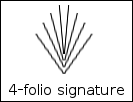
\includegraphics{signature.jpg}}
  \carboncopy{Prof. S. Mariotte, Mumford University}
  \enclosed{
    \begin{enumerate}
    \item list of course numbers that are most fequently viewed at
      our university (1pp)
    \item a list of students desiring to take an internship at
      Mumford University (2pp)
    \end{enumerate}
  }
\end{document}
%</le-example> 
% \end{verbatim}
%
% \paragraph{Example with configuration file}~\\
% Probably, one has to write many letters. The sender details will be
% most certainly valid for many an occasion. Therefore, you might want
% to consider putting this default setup in a configuration file,
% e.g. \texttt{uantwerpenletter.cfg}:
%
% \begin{verbatim}
%<*le-cfg>
%% configuration file for uantwerpenletter class
\usepackage{fontspec} % XeLaTeX/LuaTeX specific, replace by e.g.
\setmainfont{Calibri} % \usepackage{cmbright}
\sender{Prof. Walter Daems}{Senior Lecturer}
\facultyacronym{TI}
\unit{CoSys-Lab}
\address{
  Campus Groenenborger\\
  Groenenborgerlaan 171\\
  B-2020 Antwerpen\\
  BELGIUM}
\email{walter.daems}{uantwerpen.be}
\phone{+32 3 265 98 43}
\mobile{+32 499 355 115}
\returnaddress{FTI - U.301 -- Groenenborgerlaan 171, 2020 Antwerpen, BELGIUM}
%</le-cfg>
% \end{verbatim}
%
% The file can then be loaded in the preamble of your letter:
% \begin{verbatim}
% %%
%% This is file `uantwerpenletter.cls',
%% generated with the docstrip utility.
%%
%% The original source files were:
%%
%% uantwerpendocs.dtx  (with options: `le')
%% 
%% This is a generated file.
%% 
%% Copyright (C) 2013-2019  by Walter Daems <walter.daems@uantwerpen.be>
%% 
%% This work may be distributed and/or modified under the conditions of
%% the LaTeX Project Public License, either version 1.3 of this license
%% or (at your option) any later version.  The latest version of this
%% license is in:
%% 
%%    http://www.latex-project.org/lppl.txt
%% 
%% and version 1.3 or later is part of all distributions of LaTeX version
%% 2005/12/01 or later.
%% 
%% This work has the LPPL maintenance status `maintained'.
%% 
%% The Current Maintainer of this work is Walter Daems.
%% 
\NeedsTeXFormat{LaTeX2e}[1999/12/01]
\ProvidesClass{uantwerpenletter}
    [2019/04/10 v2.4 .dtx skeleton file]
\def\fileversion{2.4}
\def\filedate{2019/04/10}
\newif\if@filled
\DeclareOption{filled}{\@filledtrue}
\ExecuteOptions{a4paper,10pt,final,oneside,openright}
\ProcessOptions
\LoadClassWithOptions{letter}
\newcommand\tat{\makeatletter @\makeatother}
\setlength{\parindent}{0pt}
\addtolength{\parskip}{0.75\baselineskip}
\setcounter{secnumdepth}{3}
\RequirePackage[top=1in, bottom=1in, left=1.34in, right=1in]{geometry}
\RequirePackage[normalem]{ulem}
\RequirePackage{atbegshi}
\RequirePackage{xstring}
\RequirePackage{etoolbox}
\RequirePackage{ifthen}
\IfFileExists{shellesc.sty}{\RequirePackage{shellesc}}{}
\newcommand{\@emptymacro}{}
\RequirePackage{graphicx}
\RequirePackage{color}
\RequirePackage{tikz}
\usetikzlibrary{positioning}
\RequirePackage{eso-pic}
\RequirePackage{fancyhdr}
\definecolor{uacorpbord}{cmyk}     {0.00,1.00,0.60,0.37}
\definecolor{uacorpblue}{cmyk}     {1.00,0.25,0.00,0.50}
\definecolor{uacorplightblue}{cmyk}{1.00,0.00,0.08,0.13}
\definecolor{uacorporange}{cmyk}   {0.00,0.32,1.00,0.09}
\definecolor{uaftifresh}{cmyk}     {0.34,1.00,0.00,0.00}
\definecolor{uaftisober}{cmyk}     {0.10,1.00,0.00,0.49}
\definecolor{lightgray}{cmyk}      {0.00,0.00,0.00,0.05}
\definecolor{darkgray}{cmyk}       {0.00,0.00,0.00,0.80}
\definecolor{watermark}{cmyk}      {0.00,0.00,0.00,0.05}
\newcommand\uaname{University of Antwerp}
\newcommand\logoname{UA_HOR_ENG_CMYK}
\newcommand\footername{4E_PMS302_BR_ENG_RGB}
\newcommand\arrname{All rights reserved}
\newcommand\orname{of}
\newcommand\domainname{uantwerp.be}
\newcommand\datename{Date}
\newcommand\subjectname{Subject}
\newcommand\academicyearname{Academic year}
\newcommand\masterthesisname{Master's thesis}
\newcommand\bachelorthesisname{Bachelor's thesis}
\newcommand\supervisorsname{Supervisors}
\newcommand\juryname{Jury}
\newcommand\jurymembersname{Members}
\newcommand\jurychairmanname{Chairman}
\newcommand\bmthesisname{Thesis to obtain the degree of}
\newcommand\pthesisnamei{Thesis submitted in fulfilment of the
  requirements for the degree of}
\newcommand\pthesisnameii{at University of Antwerp}
\newcommand\@faculty{< Specify faculty using \textbackslash{}facultyacronym\{ABC\} >}
\newcommand\faccpg{
  \renewcommand\@faculty{Centre Pieter Gillis}}
\newcommand\facfbd{
  \renewcommand\@faculty{
    Faculty of Pharmaceutical, Biomedical and Veterinary Sciences}}
\newcommand\facggw{
  \renewcommand\@faculty{Faculty of Medicine and Health Sciences}}
\newcommand\insiob{
  \renewcommand\@faculty{Insitute of Development Policy}}
\newcommand\insoiw{
  \renewcommand\@faculty{Institute of Educations and Information Sciences}}
\newcommand\asoe{
  \renewcommand\@faculty{Antwerp School of Education}}
\newcommand\faclw{
  \renewcommand\@faculty{Faculty of Arts}}
\newcommand\facow{
  \renewcommand\@faculty{Faculty of Design Sciences}}
\newcommand\facsw{
  \renewcommand\@faculty{Faculty of Social Sciences}}
\newcommand\facrec{
  \renewcommand\@faculty{Faculty of Law}}
\newcommand\factew{
  \renewcommand\@faculty{Faculty of Applied Economics}}
\newcommand\facti{
  \renewcommand\@faculty{Faculty of Applied Engineering}}
\newcommand\facwet{
  \renewcommand\@faculty{Faculty of Science}}
\newcommand\weightname{Weight}
\AtBeginDocument{
  \@ifpackageloaded{babel}{
    \addto\captionsdutch{%
      \renewcommand\uaname{Universiteit Antwerpen}
      \renewcommand\logoname{UA_HOR_NED_CMYK}
      \renewcommand\footername{4E_PMS302_BR_NED_RGB}
      \renewcommand\arrname{Alle rechten voorbehouden}
      \renewcommand\orname{van}
      \renewcommand\domainname{uantwerpen.be}
      \renewcommand\subjectname{Onderwerp}%
      \renewcommand\datename{Datum}%
      \renewcommand\academicyearname{Academiejaar}
      \renewcommand\masterthesisname{Masterproef}
      \renewcommand\bachelorthesisname{Bachelorproef}
      \renewcommand\supervisorsname{Promotoren}
      \renewcommand\juryname{Jury}
      \renewcommand\jurymembersname{Leden}
      \renewcommand\jurychairmanname{Voorzitter}
      \renewcommand\bmthesisname{Proefschrift tot het behalen van de
        graad van}
      \renewcommand\pthesisnamei{Proefschrift voorgelegd tot het
        behalen van de graad van}
      \renewcommand\pthesisnameii{aan de \uaname{} te
        verdedigen door}
      \renewcommand\faccpg{
        \renewcommand\@faculty{Centrum Pieter Gillis}}
      \renewcommand\facfbd{
        \renewcommand\@faculty{
          Faculteit Farmaceutische, Biomedische en Diergeneeskundige
          Wetenschappen}}
      \renewcommand\facggw{
        \renewcommand\@faculty{Faculteit Geneeskunde en
          Gezondheidswetenschappen}}
      \renewcommand\insiob{
        \renewcommand\@faculty{Instituut voor Ontwikkelingsbeleid- en
          beheer}}
      \renewcommand\insoiw{
        \renewcommand\@faculty{Instituut voor Onderwijs- en
          Informatiewetenschappen}}
      \renewcommand\asoe{
        \renewcommand\@faculty{Antwerp School of Education}}
      \renewcommand\faclw{\renewcommand\@faculty{Faculteit
          Letteren en Wijsbegeerte}}
      \renewcommand\facow{
        \renewcommand\@faculty{Faculteit Ontwerpwetenschappen}}
      \renewcommand\facsw{
        \renewcommand\@faculty{Faculteit Sociale Wetenschappen}}
      \renewcommand\facrec{
        \renewcommand\@faculty{Faculteit Rechten}}
      \renewcommand\factew{
        \renewcommand\@faculty{Faculteit Toegepaste Economische
          Wetenschappen}}
      \renewcommand\facti{
        \renewcommand\@faculty{Faculteit Toegepaste
          Ingenieurswetenschappen}}
      \renewcommand\facwet{
        \renewcommand\@faculty{Faculteit Wetenschappen}}
      \renewcommand\weightname{Gewicht}
    }
    \addto\captionsgerman{%
      \renewcommand\uaname{Universit\"at Antwerpen}
      \renewcommand\logoname{UA_HOR_DUI_CMYK}
      \renewcommand\footername{4E_PMS302_BR_NED_RGB}
      \renewcommand\arrname{Alle Rechte vorbehalten}
      \renewcommand\orname{von}
      \renewcommand\domainname{uantwerpen.be}
      \renewcommand\subjectname{Betreff}%
      \renewcommand\datename{Datum}%
      \renewcommand\academicyearname{Akademisches Jahr}
      \renewcommand\masterthesisname{Masterdissertation}
      \renewcommand\bachelorthesisname{Bachelordissertation}
      \renewcommand\supervisorsname{Veranstalter}
      \renewcommand\juryname{Jury}
      \renewcommand\jurymembersname{Mitglieder}
      \renewcommand\jurychairmanname{Vorsitzender}
      \renewcommand\bmthesisname{Dissertation zur Erreichung des
        Grades der}
      \renewcommand\pthesisnamei{Dissertation zur Erreiching des
        Grades der}
      \renewcommand\pthesisnameii{an die \uaname}
      \renewcommand\faccpg{
        \renewcommand\@faculty{Centrum Pieter Gillis}}
      \renewcommand\facfbd{
        \renewcommand\@faculty{
          Faculteit Farmaceutische, Biomedische en Diergeneeskundige
          Wetenschappen}}
      \renewcommand\facggw{
        \renewcommand\@faculty{Faculteit Geneeskunde en
          Gezondheidswetenschappen}}
      \renewcommand\insiob{
        \renewcommand\@faculty{Instituut voor Ontwikkelingsbeleid- en
          beheer}}
      \renewcommand\insoiw{
        \renewcommand\@faculty{Instituut voor Onderwijs- en
          Informatiewetenschappen}}
      \renewcommand\asoe{
        \renewcommand\@faculty{Antwerp School of Education}}
      \renewcommand\faclw{\renewcommand\@faculty{Faculteit
          Letteren en Wijsbegeerte}}
      \renewcommand\facow{
        \renewcommand\@faculty{Faculteit Ontwerpwetenschappen}}
      \renewcommand\facsw{
        \renewcommand\@faculty{Faculteit Sociale Wetenschappen}}
      \renewcommand\facrec{
        \renewcommand\@faculty{Faculteit Rechten}}
      \renewcommand\factew{
        \renewcommand\@faculty{Faculteit Toegepaste Economische
          Wetenschappen}}
      \renewcommand\facti{
        \renewcommand\@faculty{Faculteit Toegepaste
          Ingenieurswetenschappen}}
      \renewcommand\facwet{
        \renewcommand\@faculty{Faculteit Wetenschappen}}
      \renewcommand\weightname{Gewicht}
    }
    \addto\captionsfrench{%
      \renewcommand\uaname{Universit\'e d'Anvers}
      \renewcommand\logoname{UA_HOR_FRA_CMYK}
      \renewcommand\footername{4E_PMS302_BR_ENG_RGB}
      \renewcommand\arrname{Tous les droits sont r\'eserv\'es}
      \renewcommand\orname{de}
      \renewcommand\domainname{uanvers.be}
      \renewcommand\subjectname{Objet}%
      \renewcommand\datename{Date}%
      \renewcommand\academicyearname{Ann\'ee acad\'emique}
      \renewcommand\masterthesisname{Th\`ese de master}
      \renewcommand\bachelorthesisname{Th\`ese de baccalaur\'eat}
      \renewcommand\supervisorsname{Promoteurs}
      \renewcommand\juryname{Jury}
      \renewcommand\jurymembersname{Membres}
      \renewcommand\jurychairmanname{Pr\'esident}
      \renewcommand\bmthesisname{Th\`ese \`a l'atteinte du degr\'e de}
      \renewcommand\pthesisnamei{Th\`ese Doctorale \`a l'atteinte du
        degr\'e de}
      \renewcommand\pthesisnameii{\`a l'\uaname}
      \renewcommand\faccpg{
        \renewcommand\@faculty{Centrum Pieter Gillis}}
      \renewcommand\facfbd{
        \renewcommand\@faculty{
          Faculteit Farmaceutische, Biomedische en Diergeneeskundige
          Wetenschappen}}
      \renewcommand\facggw{
        \renewcommand\@faculty{Faculteit Geneeskunde en
          Gezondheidswetenschappen}}
      \renewcommand\insiob{
        \renewcommand\@faculty{Instituut voor Ontwikkelingsbeleid- en
          beheer}}
      \renewcommand\insoiw{
        \renewcommand\@faculty{Instituut voor Onderwijs- en
          Informatiewetenschappen}}
      \renewcommand\asoe{
        \renewcommand\@faculty{Antwerp School of Education}}
      \renewcommand\faclw{\renewcommand\@faculty{Faculteit
          Letteren en Wijsbegeerte}}
      \renewcommand\facow{
        \renewcommand\@faculty{Faculteit Ontwerpwetenschappen}}
      \renewcommand\facsw{
        \renewcommand\@faculty{Faculteit Sociale Wetenschappen}}
      \renewcommand\facrec{
        \renewcommand\@faculty{Faculteit Rechten}}
      \renewcommand\factew{
        \renewcommand\@faculty{Faculteit Toegepaste Economische
          Wetenschappen}}
      \renewcommand\facti{
        \renewcommand\@faculty{Faculteit Toegepaste
          Ingenieurswetenschappen}}
      \renewcommand\facwet{
        \renewcommand\@faculty{Faculteit Wetenschappen}}
      \renewcommand\weightname{Poids}
    }
    \addto\captionsspanish{%
      \renewcommand\uaname{Universidad de Amberes}
      \renewcommand\logoname{UA_HOR_SPA_CMYK}
      \renewcommand\footername{4E_PMS302_BR_ENG_RGB}
      \renewcommand\arrname{Todos los derechos reservados}
      \renewcommand\orname{de}
      \renewcommand\domainname{uantwerp.be}
      \renewcommand\subjectname{Asunto}%
      \renewcommand\datename{Fecha}%
      \renewcommand\academicyearname{A\~no acad\'emico}
      \renewcommand\masterthesisname{Tesis de maestr\'\i{}a}
      \renewcommand\bachelorthesisname{Tesis de bachiller}
      \renewcommand\supervisorsname{Promotores}
      \renewcommand\juryname{Jurado}
      \renewcommand\jurymembersname{Miembros}
      \renewcommand\jurychairmanname{Presidente}
      \renewcommand\bmthesisname{Disertaci\'on a la consecuci\'on del
        grado de}
      \renewcommand\pthesisnamei{Disertaici\'on a la consecuci\'on del
        grado de}
      \renewcommand\pthesisnameii{a l'\uaname}
      \renewcommand\faccpg{
        \renewcommand\@faculty{Centrum Pieter Gillis}}
      \renewcommand\facfbd{
        \renewcommand\@faculty{
          Faculteit Farmaceutische, Biomedische en Diergeneeskundige
          Wetenschappen}}
      \renewcommand\facggw{
        \renewcommand\@faculty{Faculteit Geneeskunde en
          Gezondheidswetenschappen}}
      \renewcommand\insiob{
        \renewcommand\@faculty{Instituut voor Ontwikkelingsbeleid- en
          beheer}}
      \renewcommand\insoiw{
        \renewcommand\@faculty{Instituut voor Onderwijs- en
          Informatiewetenschappen}}
      \renewcommand\asoe{
        \renewcommand\@faculty{Antwerp School of Education}}
      \renewcommand\faclw{\renewcommand\@faculty{Faculteit
          Letteren en Wijsbegeerte}}
      \renewcommand\facow{
        \renewcommand\@faculty{Faculteit Ontwerpwetenschappen}}
      \renewcommand\facsw{
        \renewcommand\@faculty{Faculteit Sociale Wetenschappen}}
      \renewcommand\facrec{
        \renewcommand\@faculty{Faculteit Rechten}}
      \renewcommand\factew{
        \renewcommand\@faculty{Faculteit Toegepaste Economische
          Wetenschappen}}
      \renewcommand\facti{
        \renewcommand\@faculty{Faculteit Toegepaste
          Ingenieurswetenschappen}}
      \renewcommand\facwet{
        \renewcommand\@faculty{Faculteit Wetenschappen}}
      \renewcommand\weightname{Peso}
    }
  }
  {}
}
\newcommand{\@facultyacronym}{}
\newcommand{\facultyacronym}[1]{
  \renewcommand{\@facultyacronym}{#1}
  \AtBeginDocument{
    \ifthenelse{\equal{#1}{CPG}}{\faccpg}{
    \ifthenelse{\equal{#1}{FBD}}{\facfbd}{
    \ifthenelse{\equal{#1}{GGW}}{\facggw}{
    \ifthenelse{\equal{#1}{IOB}}{\insiob}{
    \ifthenelse{\equal{#1}{IOIW}}{\insoiw}{
    \ifthenelse{\equal{#1}{ASoE}}{\asoe}{
    \ifthenelse{\equal{#1}{LW}}{\faclw}{
    \ifthenelse{\equal{#1}{OW}}{\facow}{
    \ifthenelse{\equal{#1}{SW}}{\facsw}{
    \ifthenelse{\equal{#1}{REC}}{\facrec}{
    \ifthenelse{\equal{#1}{TEW}}{\factew}{
    \ifthenelse{\equal{#1}{TI}}{\facti}{
    \ifthenelse{\equal{#1}{WET}}{\facwet}{
      \errmessage{Error: wrong faculty acronym; choose one of CPG, FBD, GGW,
        IOB, IOIW, ASoE, LW, OW, SW, REC, TEW, TI, WET}}}}}}}}}}}}}}}
}
\newcommand{\@sender}{< Specify sender using
  \textbackslash{}sender\{name\}\{role\} >}
\newcommand{\@senderrole}{~}
\newcommand{\sender}[2]{\renewcommand{\@sender}{#1}\renewcommand{\@senderrole}{#2}}
\newcommand{\@logo}{\logoname}
\newcommand{\logo}[1]{\renewcommand{\@unit}{#1}}
\newcommand{\@unit}{}
\newcommand{\unit}[1]{\renewcommand{\@unit}{#1}}
\newcommand{\@emailuser}{}
\newcommand{\@emaildomain}{}
\newcommand{\email}[2]{\renewcommand{\@emailuser}{#1}\renewcommand{\@emaildomain}{#2}}
\newcommand{\@phone}{}
\newcommand{\phone}[1]{\renewcommand{\@phone}{#1}}
\newcommand{\@fax}{}
\newcommand{\fax}[1]{\renewcommand{\@fax}{#1}}
\newcommand{\@mobile}{}
\newcommand{\mobile}[1]{\renewcommand{\@mobile}{#1}}
\newcommand{\@returnaddress}{<specify return-address using \textbackslash\{single-line-return-address\}>}
\renewcommand{\returnaddress}[1]{\renewcommand{\@returnaddress}{#1}}
\newcommand{\@to}{<Specify addressee using \textbackslash{}to\{name\}>}
\renewcommand{\to}[1]{\renewcommand{\@to}{#1}}
\newcommand{\@toorganization}{<Specify organization using
  \textbackslash{}toorganization\{\}>}
\newcommand{\toorganization}[1]{\renewcommand{\@toorganization}{#1}}
\newcommand{\@toaddress}{<Specify (multiline) destination address\\using \textbackslash{}toaddress\{\}>}
\newcommand{\toaddress}[1]{\renewcommand{\@toaddress}{#1}}
\newcommand{\@subject}{-}
\newcommand*{\subject}[1]{\renewcommand{\@subject}{#1}}
\renewcommand*{\opening}[1]{#1}
\newcommand{\@closing}{<specify a closing formula using \textbackslash{}closing\{\}>}
\renewcommand*{\closing}[1]{\renewcommand{\@closing}{#1}}
\newcommand{\@signature}{\vspace*{8ex}}
\renewcommand*{\signature}[1]{\renewcommand{\@signature}{#1}}
\newcommand{\@carboncopy}{}
\newcommand{\carboncopy}[1]{\renewcommand{\@carboncopy}{#1}}
\newcommand{\@enclosed}{}
\newcommand{\enclosed}[1]{\renewcommand{\@enclosed}{#1}}
\newcommand{\@address}{\errmessage{Please, set your multi-line address
    and contact details using the \textbackslash{}address\{\} command
    in the preamble of your document}}
\renewcommand{\address}[1]{\renewcommand{\@address}{#1}}
\lhead[]{}
\chead[]{}
\rhead[]{}
\lfoot[\small\textcolor{gray}{\@date}]{\textcolor{gray}{\@date}}
\cfoot[]{}
\rfoot[\small\textcolor{gray}{\pagename~\thepage~\orname~\pageref{lastpage}}]{\small\textcolor{gray}{\pagename~\thepage~\orname~\pageref{lastpage}}}

\renewcommand{\headrulewidth}{0pt}
\renewcommand{\footrulewidth}{0pt}
\if@filled\else
  \raggedright
\fi
\raggedbottom
\onecolumn
\newcommand\maketitle{%
  \pagestyle{fancy}
  \thispagestyle{empty}
  \begin{tikzpicture}[overlay,remember picture]
    \path (current page.north west) +(1.8cm,-1.2cm)
    node[anchor=north west] {
      \includegraphics[height=1.1cm]{\@logo}
    };
    \draw (current page.north west)
    +(1cm,-98mm) -- +(1.5cm,-98mm);
    % 90 x 45
    % pos: 20mm van kant, 15mm van onderkant
    \path (current page.north east) +(-100mm,-65mm)
    node[anchor=west,text width=80mm,align=left] {
      \scriptsize\textcolor{gray}{\uline{\@returnaddress}}\\*
      \normalsize\@to\\*
      \@toorganization\\*
      \@toaddress
    };
  \end{tikzpicture}
  \begin{tikzpicture}[overlay,remember picture]
    \path (current page.south west) +(0,-0.7cm)
    node[anchor=south west,inner sep=0pt, outer sep=0pt]
    {\includegraphics{\footername}};
  \end{tikzpicture}
  ~\\[3ex]
  \textcolor{uacorpblue}{\bf \@sender}
  \ifx\@senderrole\@emptymacro\\[1.75ex]\else \\*\@senderrole\\[1.75ex]\fi
  \@faculty
  \ifx\@unit\@emptymacro\else\\* \@unit\fi~\\[1.75ex]
  \@address\\[1.75ex]
  \ifx\@email\@emptymacro\else E \@emailuser\tat{}\@emaildomain\\\fi
  \ifx\@phone\@emptymacro\else T \@phone\\\fi
  \ifx\@fax\@emptymacro\else F \@fax\\\fi
  \ifx\@mobile\@emptymacro\else M \@mobile\\\fi
  ~\\[4ex]
  \begin{tikzpicture}[anchor=north west,align=left,outer sep=0,inner sep=0]
    \path
    (0,0) node { \scriptsize \strut
      \textcolor{gray}{\uppercase\expandafter{\datename} } }
    (4cm,0) node { \scriptsize \strut
      \textcolor{gray}{\uppercase\expandafter{\subjectname} } }
    (0,-2.5ex) node { \strut \@date }
    (4cm,-2.5ex) node[align=left] { \strut \@subject };
  \end{tikzpicture}~\\[4ex]
}
\AtEndDocument{
  \@closing\\*[3ex]\@signature~\\[3ex]
  \@sender
  \ifx\@senderrole\@emptymacro\\[8ex]\else\\*\@senderrole\\[8ex]\fi
  \setlength{\parskip}{0em}
  \ifx\@carboncopy\@emptymacro\else CC: \@carboncopy\\[4ex]\fi
  \ifx\@enclosed\@emptymacro\else ENCL: \@enclosed\fi
  \label{lastpage}
}
\endinput
%%
%% End of file `uantwerpenletter.cls'.

% \end{verbatim}
%
% After loading this configuration file, you may override some
% elements if this is appropriate.
%
% You may also consider using multiple configuration files in case you
% have multiple roles in the university. Just make sure they are on your
% \LaTeX\ search path.
%
% \subsubsection{\texttt{uantwerpenexam}}
%
% Below you can find two examples:
% \begin{itemize}
% \item A single column layout (single language) exam
% \item A double column layout (English-Dutch) exam
% \end{itemize}
% If you require more language combinations, aks the author to
% implement this.
%
% \paragraph{Single column}
% \begin{verbatim}
%<*ex-example1> 
\documentclass[a4paper,10pt]{uantwerpenexam}
\usepackage{newpxtext} % demonstration of some fine font packages
\usepackage{newpxmath}
\usepackage{enumitem}
\usepackage[dutch]{babel} % last language loaded will
                          % determine logo version (change to
                          % [dutch] for a monolingual version)
\course{19876FTIDUM}{5-Bistrologie}
\author{Walter Daems}
\facultyacronym{TI}
\programme{BA}{IW}{EI}
\academicyear{2017-2018}
\exampart{Schriftelijk Examen}
\examgroupnumber{1 (eerste examenkans-inhaal)}
\examdate{2018-01-29}
\examlength{4h}
\tstart{08h30}
\tend{12h30}
\rooms{G.U.025}
\extrainfo[firstpage]{
  Belangrijke informatie:\\\par
  Het volledige Onderwijs- en Examenregelement (OER) is van toepassing
  op dit examen. 
  Toch wil ik vooraf nog een aantal regels duidelijk stellen:
  \begin{enumerate}
  \item Mogen op je tafeltje aanwezig zijn:
    (1) schrijfgerief, los d.w.z. \emph{niet} in een pennenzak (geen
    papier; er zit examenpapier bij de opgaven), 
    (2) je rekenmachine (zonder alfanumerieke data en zonder
    geheugenkaarten),
    (3) het formularium.
  \item Volledig \emph{verboden te gebruiken}: alle apparatuur met
    geheugen- of communicatiefunctionaliteit zoals GSM, smartphone,
    smartwatch, muziekspeler, \ldots
    Je tas staat vooraan in het lokaal. Hang je jas aan de kapstok of
    leg hem bij je tas.
  \item Schrijf je naam op het titelblad van de opgave in het daartoe
    voorziene vak. Op de andere bladen schrijf je je naam
    \emph{niet}. Je examenopgave heeft een uniek nummer dat toelaat het
    te identificeren.
  \item Op het einde van het examen geef je \emph{alle} bladen weer af
    aan de aanwezige docent.
  \end{enumerate}
  Succes!
}
\studentnr{127}
\setmcsymbol{\bigcirc}

\begin{document}
\maketitle
\question{[VLATOP-BISTRO]}
\questionweight{3}

Geef de eerste vijf laureaten van de VLATOP-bistro
competitie.

\question{[BECHAMEL]}
\questionweight{7}

Welk van de onderstaande ingredi\"enten hoort niet thuis in
  een b\'echamel saus:
\mc{Melk}
\mc{Boter}
\mc{Bloem}
\mc{Eieren}
\mc{Suiker}

\insertsolutionspagepartial{2}

\insertsolutionspage{}
\clearpage

\question{[BISTROCULTURE-1]}
\questionweight{10}

\begin{enumerate}[label=\alph*)]
\item Bespreek de evolutie van de Noord-Europese bistrocultuur
  gedurende de laatste vijftig jaar.
\item Breng dit in relatie tot de
  opkomst van de georganiseerde recensies zoals die van Michelin en
  Gault-Millau.
\end{enumerate}

\insertsolutionspagepartial{23}
\foreach \i in {1,2,3} {
  \insertsolutionspage{}
}
\foreach \i in {1,2} {
  \insertsolutionspage{Kladpapier}
}
\end{document}
%</ex-example1>
% \end{verbatim}
%
% \paragraph{Two columns}
% \begin{verbatim}
%<*ex-example2> 
\documentclass[a4paper,10pt]{uantwerpenexam}
\usepackage{newpxtext} % demonstration of some fine font packages
\usepackage{newpxmath}
\usepackage{enumitem}
\usepackage[dutch,english]{babel} % last language loaded will
                                  % determine logo version (change to
                                  % [dutch] for a monolingual version)
\course{19876FTIDUM}{5-Bistrology}
\author{Walter Daems}
\facultyacronym{TI}
\programme{BA}{IW}{EI}
\academicyear{2017-2018}
\exampart{Written Exam}
\examgroupnumber{1 (eerste examenkans-inhaal)}
\examdate{2018-01-29}
\examlength{4h}
\tstart{08h30}
\tend{12h30}
\rooms{G.U.025}
\extrainfo{
  \engdut{
    Important information:\\\par
    The Education and Examination Regulations (EER) hold for this
    examination in full.
    However, before starting, I'd like to set some rules straight:
  }
  {
    Belangrijke informatie:\\\par
    Het volledige Onderwijs- en Examenregelement (OER) is van toepassing
    op dit examen. 
    Toch wil ik vooraf nog een aantal regels duidelijk stellen:
  }
  \engdut{
    \begin{itemize}
    \item \emph{Can be used:} (1) writing gear (\emph{not} in a pencil
      case); you don't need paper; there's plenty of paper in your exam
      copy;
      (2) your calculator (without alphanumerical data and without memory
      cards); (3) the formula collection.
    \end{itemize}
  }
  {
    \begin{itemize}
    \item Mogen op je tafeltje aanwezig zijn:
      (1) schrijfgerief, los d.w.z. \emph{niet} in een pennenzak (geen
      papier; er zit examenpapier bij de opgaven), 
      (2) je rekenmachine (zonder alfanumerieke data en zonder
      geheugenkaarten),
      (3) het formularium.
    \end{itemize}
  }
  \engdut{
    \begin{itemize}
    \item \emph{May not be used:} all equipment with memory or
      communications facilities, like cell phones, smart phones, smart
      watches, music players, \ldots
      Your bag must be put in the front of the room. Put your coat on the
      hallstand or next to your bag.
    \end{itemize}
  }
  {
    \begin{itemize}
    \item Volledig \emph{verboden te gebruiken}: alle apparatuur met
      geheugen- of communicatiefunctionaliteit zoals GSM, smartphone,
      smartwatch, muziekspeler, \ldots
      Je tas staat vooraan in het lokaal. Hang je jas aan de kapstok of
      leg hem bij je tas.
    \end{itemize}
  }
  \engdut{
    \begin{itemize}
    \item Write your name on the title page. Don't write your name on
      the subsequent pages. Your copy has a unique number to identify it
      as yours.
    \end{itemize}
  }
  {
    \begin{itemize}
    \item Schrijf je naam op het titelblad van de opgave in het daartoe
      voorziene vak. Op de andere bladen schrijf je je naam
      \emph{niet}. Je examenopgave heeft een uniek nummer dat toelaat het
      te identificeren.
    \end{itemize}
  }
  \engdut{
    \begin{itemize}
    \item Take your time to \emph{answer all questions in writing}. The
      point weights are listed above every question. Be complete in your
      answer, but stick to the point. Take into account the available time.
    \end{itemize}
  }
  {
    \begin{itemize}
    \item Neem je tijd om \emph{alle vragen schriftelijk te
        beantwoorden}. Het puntengewicht van een vraag is bovenaan de vraag
      op de opgavebladen vermeld. Wees volledig in je antwoord, maar ter
      zake. Houd rekening met de beschikbare tijd.
    \end{itemize}
  }
  \engdut{
    \begin{itemize}
    \item Hand in \emph{all} papers to the staff member on duty, at the
      end of the examination.
    \end{itemize}
    Success!
  }
  {
    \begin{itemize}
    \item Op het einde van het examen geef je \emph{alle} bladen weer af
      aan de aanwezige docent.
    \end{itemize}
    Succes!
  }
  \clearpage
}

\studentnr{29}
\begin{document}
\maketitle
\question{[VLATOP-BISTRO]}
\questionweight{3}

\engdut{
  Write down the first five laureates of the VALTOP-bistro competition.
}
{
  Geef de eerste vijf laureaten van de VLATOP-bistro
  competitie.
}

\question{[BECHAMEL]}
\questionweight{7}

\engdut{
  Which of the ingredients below does not belong in a b\'echamel
  sauce:
}
{
  Welk van de onderstaande ingredi\"enten hoort niet thuis in
  een b\'echamel saus:
}
\engdutmc{Milk}{Melk}
\engdutmc{Butter}{Boter}
\engdutmc{Flower}{Bloem}
\engdutmc{Eggs}{Eieren}
\engdutmc{Sugar}{Suiker}

\insertsolutionspagepartial{20}

\insertsolutionspage{}
\clearpage

\question{[BISTROCULTURE-1]}
\questionweight{10}

\engdut{
  \begin{enumerate}[label=\alph*)]
  \item Discuss the evolution of the Northern European bistro culture during
    the latest fifty years.
  \item Relate this to the rise of organized reviews
    like the ones of Michelin and Gault-Millau.
  \end{enumerate}
}
{
  \begin{enumerate}[label=\alph*)]
  \item Bespreek de evolutie van de Noord-Europese bistrocultuur
    gedurende de laatste vijftig jaar.
  \item Breng dit in relatie tot de
    opkomst van de georganiseerde recensies zoals die van Michelin en
    Gault-Millau.
  \end{enumerate}
}

\insertsolutionspagepartial{22.5}
\foreach \i in {1,2,3} {
  \insertsolutionspage{}
}
\foreach \i in {1,2} {
  \insertsolutionspage{Scrap/Klad}
}
\end{document}
%</ex-example2>
% \end{verbatim}
%
% \StopEventually{\clearpage\PrintChanges\clearpage\PrintIndex}
% 
% \section{Implementation}
% 
% \subsection{Class inheritance}
% 
% 
% For convenience, we'll derive from the standard \LaTeX{} |book|, 
% |letter| and |article| class. 
% 
% \changes{v1.0}{2013/05/11}{Added option titlepagetableonly}
% \changes{v1.0}{2013/05/11}{Added option titlepagenoartwork}
% \changes{v1.0}{2013/05/11}{Added option qr}
% \changes{v1.4}{2016/01/07}{Implemented letter class}
% \changes{v1.9}{2018/03/02}{Implemented uantwerpenexam class}
% \changes{v2.0}{2018/03/02}{Implemented uantwerpenphdthesis class}
%
% Before loading the class, we provide the extra options.
% 
%    \begin{macrocode}
%<*ct>      
\newif\if@copyright
\DeclareOption{copyright}{\@copyrighttrue}
\newif\if@qr
\DeclareOption{qr}{\@qrtrue}
%</ct>
%    \end{macrocode}
%
%    \begin{macrocode}
%<*ct|bmt|pt>
\newif\if@titlepagenoartwork
\DeclareOption{titlepagenoartwork}{\@titlepagenoartworktrue}
\newif\if@titlepagetableonly
\DeclareOption{titlepagetableonly}{\@titlepagetableonlytrue}
%</ct|bmt|pt>
%<*ct|bmt|pt|le>
\newif\if@filled
\DeclareOption{filled}{\@filledtrue}
%</ct|bmt|pt|le>
%<*ex>
\newif\if@examiner
\DeclareOption{examiner}{\@examinertrue}
%</ex>
%    \end{macrocode}
%
%
% We execute some standard options:
% We load the |book| class for course texts and master theses.
%    \begin{macrocode}
%<*ct|bmt|pt> 
\ExecuteOptions{a4paper,11pt,final,oneside,openright}
\ProcessOptions
\LoadClassWithOptions{book}
%</ct|bmt|pt>
% We load the |letter| class for letters
%<*le> 
\ExecuteOptions{a4paper,10pt,final,oneside,openright}
\ProcessOptions
\LoadClassWithOptions{letter}
\newcommand\tat{\makeatletter @\makeatother}
%</le>
% We load the |article| class for exams
%<*ex>
\ExecuteOptions{a4paper,twoside,10pt}
\ProcessOptions
\LoadClassWithOptions{article}
%</ex>
%    \end{macrocode}
% 
% \subsection{Modern typesetting}
% Let's force some modern typesetting without paragraph indentation
% and with a decent paragraph spacing.
% 
%    \begin{macrocode}
%<*ct|bmt|pt|le|ex>      
\setlength{\parindent}{0pt}
\addtolength{\parskip}{0.75\baselineskip}
\setcounter{secnumdepth}{3}
%</ct|bmt|pt|le|ex> 
%    \end{macrocode}
% 
% \subsection{Auxiliary packages}
% Reinventing the wheel is a waste of time, let's preload some
% appropriate auxiliary packages that have proven their value.
%
% \subsubsection{Geometry}
% Let's reduce the margins to 1 inch each.
%    \begin{macrocode}
%<*ct|bmt|pt|ex>      
\RequirePackage[top=1in, bottom=1in, left=1in, right=1in]{geometry}
%</ct|bmt|pt|ex> 
%<*le>      
\RequirePackage[top=1in, bottom=1in, left=1.34in, right=1in]{geometry}
\RequirePackage[normalem]{ulem}
\RequirePackage{atbegshi}
%</le> 
%    \end{macrocode}
% 
% \subsubsection{Font packages}
% Note that the use of cmbright is no
% longer imposed (as of v1.3). Using a good font is now up to the
% user. The packages 'newpxtext/newpxmath' and 'cmbright' are highly
% recommended.
% For writing letters, 'Calibri' is the official font of the
% University of Antwerp.
% \changes{v1.2}{2014/08/22}{Added lmodern package to please MikTeX}
% \changes{v1.3}{2015/12/31}{Abandoned use of cmbright - no more
% font dictatorship for theses and courses}
%    \begin{macrocode}
%<*ct|bmt|pt|le>      
% no more font code
%</ct|bmt|pt|le>
%    \end{macrocode}
%
% \subsubsection{Boilerplate packages}
% 
% Some boilerplate packages and an empty macro to test against
% (using|\ifx|)
% \changes{v1.8}{2017/01/08}{Added missing packages ifmtarg and
% shellesc}
% \changes{v1.81}{2017/01/09}{Apparently shellesc is still missing from
% quite a number of installations, therefore, conditional loading}
% \changes{v1.9}{2018/03/02}{Added etoolbox for convenience reasons}
% \changes{v2.0}{2018/03/14}{Removed package ifmtarg because unreliable}
%    \begin{macrocode}
%<*ct|bmt|pt|le|ex>
\RequirePackage{xstring}
\RequirePackage{etoolbox}
\RequirePackage{ifthen}
\IfFileExists{shellesc.sty}{\RequirePackage{shellesc}}{}
\newcommand{\@emptymacro}{}
%</ct|bmt|pt|le|ex> 
%    \end{macrocode}
% 
% \subsubsection{Graphics packages}
% 
% Graphics packages that are required for the title page, but may come
% in handy for regular use as well.
%
% Some packages for coursetext and bamathesis:
% \changes{v1.3}{2015/12/31}{Added inclusion of background package}
%    \begin{macrocode}
%<*ct|bmt|pt|le|ex>      
\RequirePackage{graphicx}
\RequirePackage{color}
\RequirePackage{tikz}
\usetikzlibrary{positioning}
\RequirePackage{eso-pic}
%</ct|bmt|pt|le|ex>
%<*ct>
\if@copyright
\RequirePackage[firstpage=false,contents={Copyright University of Antwerp, All Rights Reserved},color=lightgray,scale=3]{background}
\fi
%</ct>
%<*pt>
\usepackage{ean13isbn} 
%</pt>
%    \end{macrocode}
%
% In uantwerpencoursetext we also want to generate a qr code.
% Therefore we load the |pst-barcode| and |auto-pst-pdf| package.
% In this case you must enable 'write18' or 'shell-escape' for your
% \LaTeX{} compiler. Check your documention on how to do so!
%
%    \begin{macrocode}
%<*ct>
\if@qr
\RequirePackage{auto-pst-pdf}
\RequirePackage{pst-barcode}
\fi
%</ct>
%    \end{macrocode}
%
% \subsubsection{Header/Footer}
% 
% The de-facto standard for headers and footers:
%    \begin{macrocode}
%<*ct|bmt|pt|le|ex>      
\RequirePackage{fancyhdr}
%</ct|bmt|pt|le|ex> 
%    \end{macrocode}
% 
% \subsection{Colors}
%
%    \begin{macrocode}
%<*ct|bmt|pt|le|ex> 
\definecolor{uacorpbord}{cmyk}     {0.00,1.00,0.60,0.37}
\definecolor{uacorpblue}{cmyk}     {1.00,0.25,0.00,0.50}
\definecolor{uacorplightblue}{cmyk}{1.00,0.00,0.08,0.13}
\definecolor{uacorporange}{cmyk}   {0.00,0.32,1.00,0.09}
\definecolor{uaftifresh}{cmyk}     {0.34,1.00,0.00,0.00}
\definecolor{uaftisober}{cmyk}     {0.10,1.00,0.00,0.49}
\definecolor{lightgray}{cmyk}      {0.00,0.00,0.00,0.05}
\definecolor{darkgray}{cmyk}       {0.00,0.00,0.00,0.80}
\definecolor{watermark}{cmyk}      {0.00,0.00,0.00,0.05}
%</ct|bmt|pt|le|ex>
%    \end{macrocode}
%
% \subsection{Babel provisions}
%
% \changes{v1.7}{2016/05/01}{Added babel tags of elements
% of master's thesis title page}
%    \begin{macrocode}
%<*ct|bmt|pt|le|ex>
\newcommand\uaname{University of Antwerp}
\newcommand\logoname{UA_HOR_ENG_CMYK}
\newcommand\footername{4E_PMS302_BR_ENG_RGB}
\newcommand\arrname{All rights reserved}
\newcommand\orname{of}
\newcommand\domainname{uantwerp.be}
\newcommand\datename{Date}
\newcommand\subjectname{Subject}
\newcommand\academicyearname{Academic year}
\newcommand\masterthesisname{Master's thesis}
\newcommand\bachelorthesisname{Bachelor's thesis}
\newcommand\supervisorsname{Supervisors}
\newcommand\juryname{Jury}
\newcommand\jurymembersname{Members}
\newcommand\jurychairmanname{Chairman}
\newcommand\bmthesisname{Thesis to obtain the degree of}
\newcommand\pthesisnamei{Thesis submitted in fulfilment of the
  requirements for the degree of}
\newcommand\pthesisnameii{at University of Antwerp}
\newcommand\@faculty{< Specify faculty using \textbackslash{}facultyacronym\{ABC\} >}
\newcommand\faccpg{
  \renewcommand\@faculty{Centre Pieter Gillis}}
\newcommand\facfbd{
  \renewcommand\@faculty{
    Faculty of Pharmaceutical, Biomedical and Veterinary Sciences}}
\newcommand\facggw{
  \renewcommand\@faculty{Faculty of Medicine and Health Sciences}} 
\newcommand\insiob{
  \renewcommand\@faculty{Insitute of Development Policy}}
\newcommand\insoiw{
  \renewcommand\@faculty{Institute of Educations and Information Sciences}}
\newcommand\asoe{
  \renewcommand\@faculty{Antwerp School of Education}}
\newcommand\faclw{
  \renewcommand\@faculty{Faculty of Arts}}
\newcommand\facow{
  \renewcommand\@faculty{Faculty of Design Sciences}}
\newcommand\facsw{
  \renewcommand\@faculty{Faculty of Social Sciences}}
\newcommand\facrec{
  \renewcommand\@faculty{Faculty of Law}}
\newcommand\factew{
  \renewcommand\@faculty{Faculty of Applied Economics}} 
\newcommand\facti{
  \renewcommand\@faculty{Faculty of Applied Engineering}}
\newcommand\facwet{
  \renewcommand\@faculty{Faculty of Science}}
\newcommand\weightname{Weight}
\AtBeginDocument{
  \@ifpackageloaded{babel}{
    \addto\captionsdutch{%
      \renewcommand\uaname{Universiteit Antwerpen}
      \renewcommand\logoname{UA_HOR_NED_CMYK}
      \renewcommand\footername{4E_PMS302_BR_NED_RGB}
      \renewcommand\arrname{Alle rechten voorbehouden}
      \renewcommand\orname{van}
      \renewcommand\domainname{uantwerpen.be}
      \renewcommand\subjectname{Onderwerp}%
      \renewcommand\datename{Datum}%
      \renewcommand\academicyearname{Academiejaar}
      \renewcommand\masterthesisname{Masterproef}
      \renewcommand\bachelorthesisname{Bachelorproef}
      \renewcommand\supervisorsname{Promotoren}
      \renewcommand\juryname{Jury}
      \renewcommand\jurymembersname{Leden}
      \renewcommand\jurychairmanname{Voorzitter}
      \renewcommand\bmthesisname{Proefschrift tot het behalen van de
        graad van}
      \renewcommand\pthesisnamei{Proefschrift voorgelegd tot het
        behalen van de graad van}
      \renewcommand\pthesisnameii{aan de \uaname{} te
        verdedigen door}
      \renewcommand\faccpg{
        \renewcommand\@faculty{Centrum Pieter Gillis}}
      \renewcommand\facfbd{
        \renewcommand\@faculty{
          Faculteit Farmaceutische, Biomedische en Diergeneeskundige
          Wetenschappen}} 
      \renewcommand\facggw{
        \renewcommand\@faculty{Faculteit Geneeskunde en
          Gezondheidswetenschappen}} 
      \renewcommand\insiob{
        \renewcommand\@faculty{Instituut voor Ontwikkelingsbeleid- en
          beheer}} 
      \renewcommand\insoiw{
        \renewcommand\@faculty{Instituut voor Onderwijs- en
          Informatiewetenschappen}}
      \renewcommand\asoe{
        \renewcommand\@faculty{Antwerp School of Education}}
      \renewcommand\faclw{\renewcommand\@faculty{Faculteit
          Letteren en Wijsbegeerte}}
      \renewcommand\facow{
        \renewcommand\@faculty{Faculteit Ontwerpwetenschappen}}
      \renewcommand\facsw{
        \renewcommand\@faculty{Faculteit Sociale Wetenschappen}}
      \renewcommand\facrec{
        \renewcommand\@faculty{Faculteit Rechten}}
      \renewcommand\factew{
        \renewcommand\@faculty{Faculteit Toegepaste Economische
          Wetenschappen}} 
      \renewcommand\facti{
        \renewcommand\@faculty{Faculteit Toegepaste
          Ingenieurswetenschappen}} 
      \renewcommand\facwet{
        \renewcommand\@faculty{Faculteit Wetenschappen}}
      \renewcommand\weightname{Gewicht}
    }
    \addto\captionsgerman{%
      \renewcommand\uaname{Universit\"at Antwerpen}
      \renewcommand\logoname{UA_HOR_DUI_CMYK}
      \renewcommand\footername{4E_PMS302_BR_NED_RGB}
      \renewcommand\arrname{Alle Rechte vorbehalten}
      \renewcommand\orname{von}
      \renewcommand\domainname{uantwerpen.be}
      \renewcommand\subjectname{Betreff}%
      \renewcommand\datename{Datum}%
      \renewcommand\academicyearname{Akademisches Jahr}
      \renewcommand\masterthesisname{Masterdissertation}
      \renewcommand\bachelorthesisname{Bachelordissertation}
      \renewcommand\supervisorsname{Veranstalter}
      \renewcommand\juryname{Jury}
      \renewcommand\jurymembersname{Mitglieder}
      \renewcommand\jurychairmanname{Vorsitzender}
      \renewcommand\bmthesisname{Dissertation zur Erreichung des
        Grades der}
      \renewcommand\pthesisnamei{Dissertation zur Erreiching des
        Grades der}
      \renewcommand\pthesisnameii{an die \uaname}
      \renewcommand\faccpg{
        \renewcommand\@faculty{Centrum Pieter Gillis}}
      \renewcommand\facfbd{
        \renewcommand\@faculty{
          Faculteit Farmaceutische, Biomedische en Diergeneeskundige
          Wetenschappen}} 
      \renewcommand\facggw{
        \renewcommand\@faculty{Faculteit Geneeskunde en
          Gezondheidswetenschappen}} 
      \renewcommand\insiob{
        \renewcommand\@faculty{Instituut voor Ontwikkelingsbeleid- en
          beheer}} 
      \renewcommand\insoiw{
        \renewcommand\@faculty{Instituut voor Onderwijs- en
          Informatiewetenschappen}}
      \renewcommand\asoe{
        \renewcommand\@faculty{Antwerp School of Education}}
      \renewcommand\faclw{\renewcommand\@faculty{Faculteit
          Letteren en Wijsbegeerte}}
      \renewcommand\facow{
        \renewcommand\@faculty{Faculteit Ontwerpwetenschappen}}
      \renewcommand\facsw{
        \renewcommand\@faculty{Faculteit Sociale Wetenschappen}}
      \renewcommand\facrec{
        \renewcommand\@faculty{Faculteit Rechten}}
      \renewcommand\factew{
        \renewcommand\@faculty{Faculteit Toegepaste Economische
          Wetenschappen}} 
      \renewcommand\facti{
        \renewcommand\@faculty{Faculteit Toegepaste
          Ingenieurswetenschappen}} 
      \renewcommand\facwet{
        \renewcommand\@faculty{Faculteit Wetenschappen}}
      \renewcommand\weightname{Gewicht}
    }
    \addto\captionsfrench{%
      \renewcommand\uaname{Universit\'e d'Anvers}
      \renewcommand\logoname{UA_HOR_FRA_CMYK}
      \renewcommand\footername{4E_PMS302_BR_ENG_RGB}
      \renewcommand\arrname{Tous les droits sont r\'eserv\'es}
      \renewcommand\orname{de}
      \renewcommand\domainname{uanvers.be}
      \renewcommand\subjectname{Objet}%
      \renewcommand\datename{Date}%
      \renewcommand\academicyearname{Ann\'ee acad\'emique}
      \renewcommand\masterthesisname{Th\`ese de master}
      \renewcommand\bachelorthesisname{Th\`ese de baccalaur\'eat}
      \renewcommand\supervisorsname{Promoteurs} 
      \renewcommand\juryname{Jury}
      \renewcommand\jurymembersname{Membres}
      \renewcommand\jurychairmanname{Pr\'esident}
      \renewcommand\bmthesisname{Th\`ese \`a l'atteinte du degr\'e de}
      \renewcommand\pthesisnamei{Th\`ese Doctorale \`a l'atteinte du
        degr\'e de}
      \renewcommand\pthesisnameii{\`a l'\uaname}
      \renewcommand\faccpg{
        \renewcommand\@faculty{Centrum Pieter Gillis}}
      \renewcommand\facfbd{
        \renewcommand\@faculty{
          Faculteit Farmaceutische, Biomedische en Diergeneeskundige
          Wetenschappen}} 
      \renewcommand\facggw{
        \renewcommand\@faculty{Faculteit Geneeskunde en
          Gezondheidswetenschappen}} 
      \renewcommand\insiob{
        \renewcommand\@faculty{Instituut voor Ontwikkelingsbeleid- en
          beheer}} 
      \renewcommand\insoiw{
        \renewcommand\@faculty{Instituut voor Onderwijs- en
          Informatiewetenschappen}}
      \renewcommand\asoe{
        \renewcommand\@faculty{Antwerp School of Education}}
      \renewcommand\faclw{\renewcommand\@faculty{Faculteit
          Letteren en Wijsbegeerte}}
      \renewcommand\facow{
        \renewcommand\@faculty{Faculteit Ontwerpwetenschappen}}
      \renewcommand\facsw{
        \renewcommand\@faculty{Faculteit Sociale Wetenschappen}}
      \renewcommand\facrec{
        \renewcommand\@faculty{Faculteit Rechten}}
      \renewcommand\factew{
        \renewcommand\@faculty{Faculteit Toegepaste Economische
          Wetenschappen}} 
      \renewcommand\facti{
        \renewcommand\@faculty{Faculteit Toegepaste
          Ingenieurswetenschappen}} 
      \renewcommand\facwet{
        \renewcommand\@faculty{Faculteit Wetenschappen}}
      \renewcommand\weightname{Poids}
    }
    \addto\captionsspanish{%
      \renewcommand\uaname{Universidad de Amberes}
      \renewcommand\logoname{UA_HOR_SPA_CMYK}
      \renewcommand\footername{4E_PMS302_BR_ENG_RGB}
      \renewcommand\arrname{Todos los derechos reservados}
      \renewcommand\orname{de}
      \renewcommand\domainname{uantwerp.be}
      \renewcommand\subjectname{Asunto}%
      \renewcommand\datename{Fecha}%
      \renewcommand\academicyearname{A\~no acad\'emico}
      \renewcommand\masterthesisname{Tesis de maestr\'\i{}a}
      \renewcommand\bachelorthesisname{Tesis de bachiller}
      \renewcommand\supervisorsname{Promotores}
      \renewcommand\juryname{Jurado}
      \renewcommand\jurymembersname{Miembros}
      \renewcommand\jurychairmanname{Presidente}
      \renewcommand\bmthesisname{Disertaci\'on a la consecuci\'on del
        grado de}
      \renewcommand\pthesisnamei{Disertaici\'on a la consecuci\'on del
        grado de}
      \renewcommand\pthesisnameii{a l'\uaname}
      \renewcommand\faccpg{
        \renewcommand\@faculty{Centrum Pieter Gillis}}
      \renewcommand\facfbd{
        \renewcommand\@faculty{
          Faculteit Farmaceutische, Biomedische en Diergeneeskundige
          Wetenschappen}} 
      \renewcommand\facggw{
        \renewcommand\@faculty{Faculteit Geneeskunde en
          Gezondheidswetenschappen}} 
      \renewcommand\insiob{
        \renewcommand\@faculty{Instituut voor Ontwikkelingsbeleid- en
          beheer}} 
      \renewcommand\insoiw{
        \renewcommand\@faculty{Instituut voor Onderwijs- en
          Informatiewetenschappen}}
      \renewcommand\asoe{
        \renewcommand\@faculty{Antwerp School of Education}}
      \renewcommand\faclw{\renewcommand\@faculty{Faculteit
          Letteren en Wijsbegeerte}}
      \renewcommand\facow{
        \renewcommand\@faculty{Faculteit Ontwerpwetenschappen}}
      \renewcommand\facsw{
        \renewcommand\@faculty{Faculteit Sociale Wetenschappen}}
      \renewcommand\facrec{
        \renewcommand\@faculty{Faculteit Rechten}}
      \renewcommand\factew{
        \renewcommand\@faculty{Faculteit Toegepaste Economische
          Wetenschappen}} 
      \renewcommand\facti{
        \renewcommand\@faculty{Faculteit Toegepaste
          Ingenieurswetenschappen}} 
      \renewcommand\facwet{
        \renewcommand\@faculty{Faculteit Wetenschappen}}
      \renewcommand\weightname{Peso}
    }
  }
  {}
}
%</ct|bmt|pt|le|ex> 
%    \end{macrocode}
%
% \subsection{Tags}
% 
% \begin{macro}{\facultyacronym}
%   The |facultyacronym| sets the faculty acronym tag
%   |\@facultyacronym| that is used in the header/footer
%   information. The correct acronym also sets the faculty's name
%   correctly.
%
%    \begin{macrocode}
%<*ct|bmt|pt|le|ex>      
\newcommand{\@facultyacronym}{}
\newcommand{\facultyacronym}[1]{
  \renewcommand{\@facultyacronym}{#1}
  \AtBeginDocument{
    \ifthenelse{\equal{#1}{CPG}}{\faccpg}{
    \ifthenelse{\equal{#1}{FBD}}{\facfbd}{
    \ifthenelse{\equal{#1}{GGW}}{\facggw}{
    \ifthenelse{\equal{#1}{IOB}}{\insiob}{
    \ifthenelse{\equal{#1}{IOIW}}{\insoiw}{
    \ifthenelse{\equal{#1}{ASoE}}{\asoe}{      
    \ifthenelse{\equal{#1}{LW}}{\faclw}{
    \ifthenelse{\equal{#1}{OW}}{\facow}{
    \ifthenelse{\equal{#1}{SW}}{\facsw}{
    \ifthenelse{\equal{#1}{REC}}{\facrec}{
    \ifthenelse{\equal{#1}{TEW}}{\factew}{
    \ifthenelse{\equal{#1}{TI}}{\facti}{
    \ifthenelse{\equal{#1}{WET}}{\facwet}{
      \errmessage{Error: wrong faculty acronym; choose one of CPG, FBD, GGW,
        IOB, IOIW, ASoE, LW, OW, SW, REC, TEW, TI, WET}}}}}}}}}}}}}}}
}
%</ct|bmt|pt|le|ex>
%    \end{macrocode}
% \end{macro}
% 
% \begin{macro}{\title}
%   The |title| tag is native to \LaTeX{}. It sets the |\@title| tag
%   that will be used on the title page.
%   However, in view of the qr trouble, we fiddle a little with it.
%   In case the title contains accented characters, you also
%   need to provide a qr version in full unicode (so without the
%   traditional \LaTeX{} accented characters.)
%
%    \begin{macrocode}
%<*ct>      
\newcommand{\@qrtitle}{}
\renewcommand{\title}[1]{%
  \renewcommand\@title{#1}
  \ifx\@qrtitle\@emptymacro
  \renewcommand\@qrtitle{#1}
  \fi
}
\newcommand{\qrtitle}[1]{%
  \renewcommand\@qrtitle{#1}
}
%</ct> 
%    \end{macrocode}
% \end{macro}
% 
% \begin{macro}{\subtitle}
%   \changes{v2.1}{2018/06/20}{Added subtitle to phd text}
%   \changes{v2.1}{2018/06/20}{Ensured that subtitle is really
%   optional by adding default space value}
%   This macro sets the |\@subtitle| tag that later will be used on
%   the title page, in the header/footer and to set the appropriate
%   |hyperref| tag.
%    \begin{macrocode}
%<*bmt>
\newcommand{\@subtitle}{Master's thesis}
%</bmt>
%<*ct|pt>      
\newcommand{\@subtitle}{~}
\newcommand{\@qrsubtitle}{}
\newcommand{\subtitle}[1]{%
  \renewcommand\@subtitle{#1}
  \ifx\@qrsubtitle\@emptymacro
    \renewcommand\@qrsubtitle{#1}
  \fi
}
\newcommand{\qrsubtitle}[1]{%
  \renewcommand\@qrsubtitle{#1}
}
%</ct|pt> 
%    \end{macrocode}
% \end{macro}
%
% \begin{macro}{\shorttitle}
%   This macro sets the |\@shorttitle| tag that later will be used
%   in the |uantwerpenexam| class.
%    \begin{macrocode}
%<*ex>      
\newcommand{\@shorttitle}{}
\newcommand{\shorttitle}[1]{%
  \renewcommand\@shorttitle{#1}
}
%</ex> 
%    \end{macrocode}
% \end{macro}
% 
% \begin{macro}{\author}
%   The |author| tag is native to \LaTeX{}. It sets the |\@author|
%   tag that will be used on the title page.
%   However, in view of the qr trouble, we fiddle a little with it for
%   the |uantwerpencoursetext| class.
%   In case the title contains accented characters, you also
%   need to provide a qr version in full unicode (so without the
%   traditional \LaTeX{} accented characters.)
%
%    \begin{macrocode}
%<*ct>      
\newcommand{\@qrauthor}{}
\renewcommand{\author}[1]{%
  \renewcommand\@author{#1}
  \ifx\@qrauthor\@emptymacro
  \renewcommand\@qrauthor{#1}
  \fi
}
\newcommand{\qrauthor}[1]{%
  \renewcommand\@qrauthor{#1}
}
%</ct> 
%    \end{macrocode}
% \end{macro}
% 
% \begin{macro}{\courseversion}
%   This macro sets the |\@courseversion| tag that later will be used
%   on the title page and in the header/footer.
%    \begin{macrocode}
%<*ct>      
\newcommand{\@courseversion}{}
\newcommand{\courseversion}[1]{\renewcommand{\@courseversion}{#1}}
%</ct> 
%    \end{macrocode}
% \end{macro}
% 
% \begin{macro}{\versionyear}
%   This macro sets the |\@versionyear| tag that later will be used on
%   the title page and in the copyright message.
%    \begin{macrocode}
%<*ct>      
\newcommand{\@versionyear}{}
\newcommand{\versionyear}[1]{\renewcommand{\@versionyear}{#1}}
%</ct> 
%    \end{macrocode}
% \end{macro}
% 
% \begin{macro}{\publisher}
%   This macro sets the |\@publisher| tag that later will be used on
%   the title page.
%    \begin{macrocode}
%<*ct>      
\newcommand{\@publisher}{\uaname\\
Cursusdienst en reprografie\\
Campus Groenenborger, G.U.027\\
Groenenborgerlaan 171\\
2020 Antwerpen\\
T +32 3 265 32 15\\
F + 32 3 233 32 27\\
E cursusdienst.cgb@uantwerpen.be}
\newcommand{\publisher}[1]{\renewcommand{\@publisher}{#1}}
%</ct> 
%    \end{macrocode}
% \end{macro}
% 
% \begin{macro}{\publishercode}
%   This macro sets the |\@publishercode| tag that later will be used on
%   the title page.
%    \begin{macrocode}
%<*ct>      
\newcommand{\@publishercode}{}
\newcommand{\publishercode}[1]{\renewcommand{\@publishercode}{#1}}
%</ct> 
%    \end{macrocode}
% \end{macro}
% 
% \begin{macro}{\lecturer}
%   This macro sets many |\@lecturer| tags (max. 4) that later will be used on
%   the title page. If there is only one teaching lecturer one can
%   use the convenient shorthand without counter.
%   In case the lecturer's name contains accented characters, you also
%   need to provide a qr version in full unicode (so without the
%   traditional \LaTeX{} accented characters.)
%    \begin{macrocode}
%<*ct>
\newcommand{\@lectureri}{}
\newcommand{\@lecturerii}{}
\newcommand{\@lectureriii}{}
\newcommand{\@lectureriv}{}
\newcommand{\@qrlectureri}{}
\newcommand{\@qrlecturerii}{}
\newcommand{\@qrlectureriii}{}
\newcommand{\@qrlectureriv}{}
\newcommand{\lecturer}[1]{
  \renewcommand{\@lectureri}{#1}
  \ifx\@qrlectureri\@emptymacro
  \renewcommand\@qrlectureri{#1}
  \fi
}
\newcommand{\qrlecturer}[1]{
  \renewcommand\@qrlectureri{#1}
}
\newcommand{\lectureri}[1]{
  \renewcommand{\@lectureri}{#1}
  \ifx\@qrlectureri\@emptymacro
  \renewcommand\@qrlectureri{#1}
  \fi
}
\newcommand{\qrlectureri}[1]{
  \renewcommand\@qrlectureri{#1}
}
\newcommand{\lecturerii}[1]{
  \renewcommand{\@lecturerii}{#1}
  \ifx\@qrlecturerii\@emptymacro
  \renewcommand\@qrlecturerii{#1}
  \fi
}
\newcommand{\qrlecturerii}[1]{
  \renewcommand\@qrlecturerii{#1}
}
\newcommand{\lectureriii}[1]{
  \renewcommand{\@lectureriii}{#1}
  \ifx\@qrlectureriii\@emptymacro
  \renewcommand\@qrlectureriii{#1}
  \fi
}
\newcommand{\qrlectureriii}[1]{
  \renewcommand\@qrlectureriii{#1}
}
\newcommand{\lectureriv}[1]{
  \renewcommand{\@lectureriv}{#1}
  \ifx\@qrlectureriv\@emptymacro
  \renewcommand\@qrlectureriv{#1}
  \fi
}
\newcommand{\qrlectureriv}[1]{
  \renewcommand\@qrlectureriv{#1}
}
%</ct> 
%    \end{macrocode}
% \end{macro}
%
%
% \begin{macro}{\affiliation}
%   The |affiliation| tag allows to specify the affiliation of the author.
%    \begin{macrocode}
%<*pt>
\newcommand\@affiliation{\errmessage{Please, define the affiliation of
    the author using the \textbackslash{}affiliation command in the
  preamble of your document.}}
\newcommand\affiliation[1]{\renewcommand\@affiliation{#1}}
%</pt>
%    \end{macrocode}
% \end{macro}
%
% \begin{macro}{\supervisor}
%   This macro sets many |\@supervisor| tags (max. 4) that later will be used on
%   the title page.
%    \begin{macrocode}
%<*bmt|pt>      
\newcommand\@supervisori{\errmessage{Please define a supervisor of
    your thesiswork using the \textbackslash{}supervisori to iv
    commands} in the preamble of your document.}
\newcommand\@supervisoriaff{}
\newcommand\@supervisorii{}
\newcommand\@supervisoriiaff{}
\newcommand\@supervisoriii{}
\newcommand\@supervisoriiiaff{}
\newcommand\@supervisoriv{}
\newcommand\@supervisorivaff{}
\newcommand{\supervisori}[2]{\renewcommand\@supervisori{#1}\renewcommand\@supervisoriaff{#2}}
\newcommand{\supervisorii}[2]{\renewcommand\@supervisorii{#1}\renewcommand\@supervisoriiaff{#2}}
\newcommand{\supervisoriii}[2]{\renewcommand\@supervisoriii{#1}\renewcommand\@supervisoriiiaff{#2}}
\newcommand{\supervisoriv}[2]{\renewcommand\@supervisoriv{#1}\renewcommand\@supervisorivaff{#2}}
%</bmt|pt> 
%    \end{macrocode}
% \end{macro}
% 
% \begin{macro}{\jurychairman}
%   This macro sets the |\@jurychairman| tag that later will be used on
%   the data page.
%    \begin{macrocode}
%<*pt>      
\newcommand{\@jurychairman}{\errmessage{Please define a chairman of the jurya
  using the \textbackslash{}jurychairman command in the preamble of your document.}}
\newcommand{\@jurychairmanaff}{}
\newcommand{\jurychairman}[2]{\renewcommand{\@jurychairman}{#1}\renewcommand{\@jurychairmanaff}{#2}}
%</pt> 
%    \end{macrocode}
% \end{macro}
% 
% \begin{macro}{\jurymember}
%   This macro sets many |\@jurymember| tags (max. 6) that later will be used on
%   the data page.
%    \begin{macrocode}
%<*pt>      
\newcommand{\@jurymemberi}{\errmessage{Please define jury members
    using the \textbackslash{}jurymemberi to vi commands in the preamble of your document.}}
\newcommand\@jurymemberiaff{}
\newcommand\@jurymemberii{}
\newcommand\@jurymemberiiaff{}
\newcommand\@jurymemberiii{}
\newcommand\@jurymemberiiiaff{}
\newcommand\@jurymemberiv{}
\newcommand\@jurymemberivaff{}
\newcommand\@jurymemberv{}
\newcommand\@jurymembervaff{}
\newcommand\@jurymembervi{}
\newcommand\@jurymemberviaff{}
\newcommand{\jurymemberi}[2]{\renewcommand\@jurymemberi{#1}\renewcommand\@jurymemberiaff{#2}}
\newcommand{\jurymemberii}[2]{\renewcommand\@jurymemberii{#1}\renewcommand\@jurymemberiiaff{#2}}
\newcommand{\jurymemberiii}[2]{\renewcommand\@jurymemberiii{#1}\renewcommand\@jurymemberiiiaff{#2}}
\newcommand{\jurymemberiv}[2]{\renewcommand\@jurymemberiv{#1}\renewcommand\@jurymemberivaff{#2}}
\newcommand{\jurymemberv}[2]{\renewcommand\@jurymemberv{#1}\renewcommand\@jurymembervaff{#2}}
\newcommand{\jurymembervi}[2]{\renewcommand\@jurymembervi{#1}\renewcommand\@jurymemberviaff{#2}}
%</pt> 
%    \end{macrocode}
% \end{macro}
% 
% \begin{macro}{\phddegree}
%   This macro sets the |\@phddegree| tag that later will
%   be used on the title pages.
%
%    \begin{macrocode}
%<*pt>
\newcommand\@phddegree{\errmessage{Please, specify the offical PhD
    degree description using the \textbackslash{}phddegree macro in
    the preamble of your document.}}
\newcommand\phddegree[1]{\renewcommand\@phddegree{#1}}
%</pt>
%    \end{macrocode}
% \end{macro}
%
%
% \begin{macro}{\programme}
%   This macro sets the |\@programme| tags that later will
%   be used on the title page. The involved way of repeatedly calling
%   the renewcommand to set the tags is required for inclusion of the
%   data as QR data.
%
%    \begin{macrocode}
%<*ct|pt|ex>      
\newcommand{\@programmet}{} % type
\newcommand{\@programmec}{} % class
\newcommand{\@programmecqr}{} % class for qr code
\newcommand{\@programmes}{} % class
\newcommand{\@programmeq}{} % qualifier
\newcommand{\programme}[3]{%
    \ifthenelse{\equal{#1}{BA}}%
    {\renewcommand{\@programmet}{Bachelor of Science in de }}{%
    \ifthenelse{\equal{#1}{MA}}%
    {\renewcommand{\@programmet}{Master of Science in de }}{%
    \ifthenelse{\equal{#1}{PHD}}%
    {\renewcommand{\@programmet}{Doctor in de }}{%
    \ifthenelse{\equal{#1}{VP}}%
    {\renewcommand{\@programmet}{Voorbereidingsprogramma voor Master of Science in de }}{%
    \ifthenelse{\equal{#1}{SP}}%
    {\renewcommand{\@programmet}{Schakelprogramma voor Master of Science in de }}{%
    \ifthenelse{\equal{#1}{FREE}}%
    {}{
    \errmessage{Error in 1st arg of macro programme[3]: invalid
      programme type!}}}}}}}%
    %
    \ifthenelse{\equal{#2}{IW}}%
    {\renewcommand{\@programmec}{industri\"ele wetenschappen}
     \renewcommand{\@programmecqr}{industriële wetenschappen}}{
    \ifthenelse{\equal{#2}{}}%
    {}{
    \errmessage{{Error in 2nd arg of macro programme[3]: invalid 
      programme class! }}}}%
    %
    \ifthenelse{\equal{#3}{BK}}%
    {\renewcommand{\@programmeq}{Bouwkunde}}{%
    \ifthenelse{\equal{#3}{CH}}%
    {\renewcommand{\@programmeq}{Chemie}}{%
    \ifthenelse{\equal{#3}{BCH}}%
    {\renewcommand{\@programmeq}{Biochemie}}{%
    \ifthenelse{\equal{#3}{EM}}%
    {\renewcommand{\@programmeq}{Elektromechanica}}{%
    \ifthenelse{\equal{#3}{EI}}%
    {\renewcommand{\@programmeq}{Elektronica-ICT}}{%
    \ifthenelse{\equal{#3}{}}%
    {}{%
    \ifthenelse{\equal{#1}{FREE}}
    {\renewcommand{\@programmeq}{#3}}{
    \errmessage{Error in 3rd arg to macro programme[3]: invalid
      programme qualifier}}}}}}}}% 
    %
    \ifthenelse{\equal{#2}{IW}\and\not\equal{#3}{}}
    {\renewcommand{\@programmes}{: }}{}
}
%</ct|pt|ex> 
%    \end{macrocode}
% \end{macro}
% 
% \begin{macro}{\course}
%   Four the |coursetext| class, this macro sets many |\@coursecode|
%   and |\@course| tags (max. 4) that later will be used on the title
%   page. If there is only one course code one can use the convenient
%   shorthand without counter.
%    \begin{macrocode}
%<*ct>      
\newcommand{\@coursecodei}{}
\newcommand{\@coursecodeii}{}
\newcommand{\@coursecodeiii}{}
\newcommand{\@coursecodeiv}{}
\newcommand{\@coursei}{}
\newcommand{\@courseii}{}
\newcommand{\@courseiii}{}
\newcommand{\@courseiv}{}
\newcommand{\@qrcoursei}{}
\newcommand{\@qrcourseii}{}
\newcommand{\@qrcourseiii}{}
\newcommand{\@qrcourseiv}{}
\newcommand{\course}[2]{
  \renewcommand{\@coursecodei}{#1}
  \renewcommand{\@coursei}{#2}
  \ifx\@qrcoursei\@emptymacro
  \renewcommand{\@qrcoursei}{#2}
  \fi
}
\newcommand{\qrcourse}[1]{
  \renewcommand{\@qrcoursei}{#1}
}
\newcommand{\coursei}[2]{
  \renewcommand{\@coursecodei}{#1}
  \renewcommand{\@coursei}{#2}
  \ifx\@qrcoursei\@emptymacro
  \renewcommand{\@qrcoursei}{#2}
  \fi
}
\newcommand{\qrcoursei}[1]{
  \renewcommand{\@qrcoursei}{#1}
}
\newcommand{\courseii}[2]{
  \renewcommand{\@coursecodeii}{#1}
  \renewcommand{\@courseii}{#2}
  \ifx\@qrcourseii\@emptymacro
  \renewcommand{\@qrcourseii}{#2}
  \fi
}
\newcommand{\qrcourseii}[1]{
  \renewcommand{\@qrcourseii}{#1}
}
\newcommand{\courseiii}[2]{
  \renewcommand{\@coursecodeiii}{#1}
  \renewcommand{\@courseiii}{#2}
  \ifx\@qrcourseiii\@emptymacro
  \renewcommand{\@qrcourseiii}{#2}
  \fi
}
\newcommand{\qrcourseiii}[1]{
  \renewcommand{\@qrcourseiii}{#1}
}
\newcommand{\courseiv}[2]{
  \renewcommand{\@coursecodeiv}{#1}
  \renewcommand{\@courseiv}{#2}
  \ifx\@qrcourseiv\@emptymacro
  \renewcommand{\@qrcourseiv}{#2}
  \fi
}
\newcommand{\qrcourseiv}[1]{
  \renewcommand{\@qrcourseiv}{#1}
}
%</ct>
%    \end{macrcode}
%   For the |exam| class (assuming that an exam only holds for a
%   single course), the situation is simple and we assume only a
%   single coursecode and course name. We also don't need any of the
%   QR stamp stuff.
%    \begin{macrocode}
%<*ex>      
\newcommand{\@coursecodei}{}
\newcommand{\@coursei}{}
\newcommand{\course}[2]{
  \renewcommand{\@coursecodei}{#1}
  \renewcommand{\@coursei}{#2}
}
%</ex>
%    \end{macrocode}
% \end{macro}
% 
% \begin{macro}{\diploma}
%   This macro sets the |\@diplomalevel| and |\@diploma| tags that
%   later will be used on the title page. 
%   \changes{v1.1}{2013/05/21}{Fixed typo on programme's name
%   (e-umlaut)}
%   \changes{v1.6}{2016/02/04}{Added diploma codes}
%   \changes{v2.3}{2019/03/27}{Added diploma level}
%   \changes{v2.4}{2019/04/10}{Added code for Master EM without specialization}
%    \begin{macrocode}
%<*bmt|pt>
\newcommand{\@diplomalevel}{ERROR}
\newcommand{\@diploma}{ERROR}
\newcommand{\diploma}[1]{
  \newcommand{\MoSIW}{Master of Science in de industri\"ele wetenschappen}
  \newcommand{\BoSIW}{Bachelor of Science in de industri\"ele wetenschappen}
  \newcommand{\MoSTEW}{Master of Science in de toegepaste economische wetenschappen}
  \renewcommand{\@diploma}{
    \ifthenelse{\equal{#1}{BA-IW-BK}}
                          {\BoSIW: bouwkunde}{
    \ifthenelse{\equal{#1}{BA-IW-BCH}}
                          {\BoSIW: biochemie}{
    \ifthenelse{\equal{#1}{BA-IW-CH}}
                          {\BoSIW: chemie}{
    \ifthenelse{\equal{#1}{BA-IW-EI}}
                          {\BoSIW: elektronica-ICT}{
    \ifthenelse{\equal{#1}{BA-IW-EM}}
                          {\BoSIW: elektromechanica}{
    \ifthenelse{\equal{#1}{MA-IW-BK}}
                          {\MoSIW: bouwkunde}{
    \ifthenelse{\equal{#1}{MA-IW-BCH}}
                          {\MoSIW: biochemie}{
    \ifthenelse{\equal{#1}{MA-IW-CH}}
                          {\MoSIW: chemie}{
    \ifthenelse{\equal{#1}{MA-IW-EI}}
                          {\MoSIW: elektronica-ICT}{
    \ifthenelse{\equal{#1}{MA-IW-EI-AE}}
                          {\MoSIW:\\elektronica-ICT, afstudeerrichting automotive engineering}{
    \ifthenelse{\equal{#1}{MA-IW-EI-ICT}}
                          {\MoSIW:\\elektronica-ICT, afstudeerrichting ICT}{
    \ifthenelse{\equal{#1}{MA-IW-EM-AE}}
                          {\MoSIW:\\elektromechanica, afstudeerrichting automotive engineering}{
    \ifthenelse{\equal{#1}{MA-IW-EM-AU}}
                          {\MoSIW:\\elektromechanica, afstudeerrichting automatisering}{
    \ifthenelse{\equal{#1}{MA-IW-EM-EM}}
                          {\MoSIW:\\elektromechanica, afstudeerrichting elektromechanica}{
    \ifthenelse{\equal{#1}{MA-IW-EM-EN}}
                          {\MoSIW:\\elektromechanica, afstudeerrichting energie}{
    \ifthenelse{\equal{#1}{MA-IW-EM}}
                          {\MoSIW:\\elektromechanica}{
    \ifthenelse{\equal{#1}{MA-TEW-HI}}
                          {\MoSTEW: handelsingenieur}{
    \ifthenelse{\equal{#1}{MA-TEW-HIBI}}
                          {\MoSTEW:\\handelsingenieur in de beleidsinformatica}{
    \ifthenelse{\equal{#1}{MA-TEW-EB}}
                          {\MoSTEW: economisch beleid}{
    \ifthenelse{\equal{#1}{MA-TEW-BK}}
                          {\MoSTEW: bedrijfskunde}
    {\errmessage{Error in argument to macro diploma: must be one of
        BA-IW-XXX with XXX one of BK, BCH, CH, EI or EM, or MA-IW-XXX with XXX one of BK, BCH, CH, EI, EI-AE, EI-ICT, EM-AE, EM-AU, EM-EM, EM-EN, MA-TEW-YYY with YYY one of HI, HIBI, EB, BK! <<}}}}}}}}}}}}}}}}}}}}}
  }
  \newcommand\thesisname{ERROR}
  \IfSubStr{#1}{MA-}{\renewcommand\thesisname{\masterthesisname}}{}
  \IfSubStr{#1}{BA-}{\renewcommand\thesisname{\bachelorthesisname}}{}
}
%</bmt|pt> 
%    \end{macrocode}
% \end{macro}
% 
% \begin{macro}{\defensedate}
%   This macro sets the |\@defensedate| tags that later will
%   be used on the title page. 
%    \begin{macrocode}
%<*bmt|pt>      
\newcommand\@defensedate{ERROR}
\newcommand{\defensedate}[1]{\renewcommand\@defensedate{#1}}
%</bmt|pt> 
%    \end{macrocode}
% \end{macro}
% 
% \begin{macro}{\defenselocation}
%   This macro sets the |\@defenselocation| tags that later will
%   be used on the title page. 
%    \begin{macrocode}
%<*bmt|pt>      
\newcommand\@defenselocation{Antwerpen}
\newcommand{\defenselocation}[1]{\renewcommand\@defenselocation{#1}}
%</bmt|pt> 
%    \end{macrocode}
% \end{macro}
%
%
% \begin{macro}{\titeplageimage}
%   This macro sets the |\@titlepageimage| tags that later will
%   be used on the title page, to include the graphics.
%    \begin{macrocode}
%<*pt>      
\newcommand\@titlepageimage{}
\newcommand\titlepageimage[1]{\renewcommand\@titlepageimage{#1}}
%</pt> 
%    \end{macrocode}
% \end{macro}
%
%
% \begin{macro}{\isbn}
%   This macro sets the |\@isbn| tags that later will
%   be used on the data page. If you don't have an ISBN number, just
%   don't specify one (i.e. don't use this macro).
%    \begin{macrocode}
%<*pt>      
\newcommand{\@isbn}{}
\newcommand{\isbn}[1]{\renewcommand{\@isbn}{#1}}
%</pt> 
%    \end{macrocode}
% \end{macro}
%
% \begin{macro}{\depot}
%   This macro sets the |\@depot| tags that later will
%   be used on the data page. 
%    \begin{macrocode}
%<*pt>      
\newcommand{\@depot}{\errmessage{Please, specify a depot number using
    the \textbackslash{}depot command in your preamble.}}
\newcommand{\depot}[1]{\renewcommand{\@depot}{#1}}
%</pt> 
%    \end{macrocode}
% \end{macro}
% 
%
% \begin{macro}{\academicyear}
%   This macro sets the |\@academicyear| tag that later will be used on
%   the title page.
%    \begin{macrocode}
%<*ct|bmt|ex>      
\newcommand{\@academicyear}{XXX-YYYY}
\newcommand{\academicyear}[1]{\renewcommand{\@academicyear}{#1}}
%</ct|bmt|ex> 
%    \end{macrocode}
% \end{macro}
% 
% \begin{macro}{\copyrightnotices}
%   This macro sets the |\@copyrightnotices| tag that later will be
%   used on the back of the title page.
%    \begin{macrocode}
%<*ct>      
\newcommand{\@copyrightnotices}{}
\newcommand{\copyrightnotices}[1]{\renewcommand{\@copyrightnotices}{#1}}
%</ct> 
%    \end{macrocode}
% \end{macro}
%
% \begin{macro}{\sender}
% This macro sets the |\@sender| and |\@senderrole| tags that will be
% used in the letter's heading text.
%    \begin{macrocode}
%<*le>
\newcommand{\@sender}{< Specify sender using
  \textbackslash{}sender\{name\}\{role\} >}
\newcommand{\@senderrole}{~}
\newcommand{\sender}[2]{\renewcommand{\@sender}{#1}\renewcommand{\@senderrole}{#2}}
%</le>
%    \end{macrocode}
% \end{macro}
%
% \begin{macro}{\logo}
%   This macro sets the |\@logo| tag that will be used to load a
%   graphics file with that name.
%    \begin{macrocode}
%<*le|ex>
\newcommand{\@logo}{\logoname}
\newcommand{\logo}[1]{\renewcommand{\@unit}{#1}}
%</le|ex>
%    \end{macrocode}
% \end{macro}
%
% \begin{macro}{\unit}
%   This macro sets the |\@unit| tag that will be used in the letter's
%   heading text.
%    \begin{macrocode}
%<*le>
\newcommand{\@unit}{}
\newcommand{\unit}[1]{\renewcommand{\@unit}{#1}}
%</le>
%    \end{macrocode}
% \end{macro}
%
% \begin{macro}{\email}
%   This macro sets the |\@emailuser| and |\@emaildomain| tags that
%   will be used in the letter's heading text. This split construction
%   was used to overcome problems with the |@| sign.
%    \begin{macrocode}
%<*le>
\newcommand{\@emailuser}{}
\newcommand{\@emaildomain}{}
\newcommand{\email}[2]{\renewcommand{\@emailuser}{#1}\renewcommand{\@emaildomain}{#2}}
%</le>
%    \end{macrocode}
% \end{macro}
%
% \begin{macro}{\phone}
%   This macro sets the |\@phone| tag that will be used in the letter's
%   heading text.
%    \begin{macrocode}
%<*le>
\newcommand{\@phone}{}
\newcommand{\phone}[1]{\renewcommand{\@phone}{#1}}
%</le>
%    \end{macrocode}
% \end{macro}
%
% \begin{macro}{\fax}
%   This macro sets the |\@fax| tag that will be used in the letter's
%   heading text.
%    \begin{macrocode}
%<*le>
\newcommand{\@fax}{}
\newcommand{\fax}[1]{\renewcommand{\@fax}{#1}}
%</le>
%    \end{macrocode}
% \end{macro}
%
%
% \begin{macro}{\mobile}
%   This macro sets the |\@mobile| tag that will be used in the letter's
%   heading text.
%    \begin{macrocode}
%<*le>
\newcommand{\@mobile}{}
\newcommand{\mobile}[1]{\renewcommand{\@mobile}{#1}}
%</le>
%    \end{macrocode}
% \end{macro}
%
%
% \begin{macro}{\returnaddress}
%   This macro sets the |\@returnaddress| tag that will be used in the letter's
%   heading text (in the area of the envelope's window).
%    \begin{macrocode}
%<*le>
\newcommand{\@returnaddress}{<specify return-address using \textbackslash\{single-line-return-address\}>}
\renewcommand{\returnaddress}[1]{\renewcommand{\@returnaddress}{#1}}
%</le>
%    \end{macrocode}
% \end{macro}
%
%
% \begin{macro}{\to}
%   This macro sets the |\@to| tag that will be used in the letter's
%   heading text (in the area of the envelope's window).
%    \begin{macrocode}
%<*le>
\newcommand{\@to}{<Specify addressee using \textbackslash{}to\{name\}>}
\renewcommand{\to}[1]{\renewcommand{\@to}{#1}}
%</le>
%    \end{macrocode}
% \end{macro}
%
%
% \begin{macro}{\toorganization}
%   This macro sets the |\@toorganization| tag that will be used in
%   the letter's heading text (in the area of the envelope's window).
%    \begin{macrocode}
%<*le>
\newcommand{\@toorganization}{<Specify organization using
  \textbackslash{}toorganization\{\}>}
\newcommand{\toorganization}[1]{\renewcommand{\@toorganization}{#1}}
%</le>
%    \end{macrocode}
% \end{macro}
%
% \begin{macro}{\toaddress}
%   This macro sets the |\@toaddress| tag that will be used in
%   the letter's heading text (in the area of the envelope's window).
%    \begin{macrocode}
%<*le>
\newcommand{\@toaddress}{<Specify (multiline) destination address\\using \textbackslash{}toaddress\{\}>}
\newcommand{\toaddress}[1]{\renewcommand{\@toaddress}{#1}}
%</le>
%    \end{macrocode}
% \end{macro}
%
% \begin{macro}{\subject}
%   This macro sets the |\@subject| tag that will be used in
%   the letter's heading text.
%    \begin{macrocode}
%<*le>
\newcommand{\@subject}{-}
\newcommand*{\subject}[1]{\renewcommand{\@subject}{#1}}
%</le>
%    \end{macrocode}
% \end{macro}
%
% \begin{macro}{\opening}
%   This macro is much a do about nothing, but I prefer to do it this
%   way for historic reasons.
%    \begin{macrocode}
%<*le>
\renewcommand*{\opening}[1]{#1}
%</le>
%    \end{macrocode}
% \end{macro}
%
% \begin{macro}{\closing}
%   This macro sets the |\@closing| tag that will be used to finish
%   the letter.
%    \begin{macrocode}
%<*le>
\newcommand{\@closing}{<specify a closing formula using \textbackslash{}closing\{\}>}
\renewcommand*{\closing}[1]{\renewcommand{\@closing}{#1}}
%</le>
%    \end{macrocode}
% \end{macro}
%
% \begin{macro}{\signature}
% \changes{v1.8}{2017/01/08}{Added signature}
%   This macro sets the |\@signature| tag that will be used to finish
%   the letter. By default this corresponds to a decent amount of vertical white space
%    \begin{macrocode}
%<*le>
\newcommand{\@signature}{\vspace*{8ex}}
\renewcommand*{\signature}[1]{\renewcommand{\@signature}{#1}}
%</le>
%    \end{macrocode}
% \end{macro}
% 
%
% \begin{macro}{\carboncopy}
%   This macro will set the |\@carboncopy| tag that will be used in
%   the trailer of the letter.
%    \begin{macrocode}
%<*le>
\newcommand{\@carboncopy}{}
\newcommand{\carboncopy}[1]{\renewcommand{\@carboncopy}{#1}}
%</le>
%    \end{macrocode}
% \end{macro}
%
% \begin{macro}{\enclosed}
%   This macro will set the |\@enclosed| tag that will be used in
%   the trailer of the letter.
%    \begin{macrocode}
%<*le>
\newcommand{\@enclosed}{}
\newcommand{\enclosed}[1]{\renewcommand{\@enclosed}{#1}}
%</le>
%    \end{macrocode}
% \end{macro}
%
% \begin{macro}{\address}
%   This macro will set the |\@address| tag that will be used in
%   the letter's heading text (in the area of the envelope's window).
%    \begin{macrocode}
%<*pt|le>
\newcommand{\@address}{\errmessage{Please, set your multi-line address
    and contact details using the \textbackslash{}address\{\} command
    in the preamble of your document}}
%</pt|le>
%<le>\renewcommand{\address}[1]{\renewcommand{\@address}{#1}}
%<pt>\newcommand{\address}[1]{\renewcommand{\@address}{#1}}
%    \end{\macrocode}
% \end{macro}
%
% \begin{macro}{\exampart}
%   This macro will set the |\@examgropunumber| tag that will be used on
%   the exam title page.
%    \begin{macrocode}
%<*ex>
\newcommand{\@exampart}{}
\newcommand{\exampart}[1]{\renewcommand{\@exampart}{#1}}
%</ex>
%    \end{macrocode}
% \end{macro}
%
% \begin{macro}{\examgroupnumber}
%   This macro will set the |\@examgroupnumber| tag that will be used on
%   the exam title page.
%    \begin{macrocode}
%<*ex>
\newcommand{\@examgroupnumber}{}
\newcommand{\examgroupnumber}[1]{\renewcommand{\@examgroupnumber}{#1}}
%</ex>
%    \end{macrocode}
% \end{macro}
%
% \begin{macro}{\examdate}
%   This macro will set the |\@examdate| tag that will be used on
%   the exam title page.
%    \begin{macrocode}
%<*ex>
\newcommand{\@examdate}{TBD}
\newcommand{\examdate}[1]{\renewcommand{\@examdate}{#1}}
%</ex>
%    \end{macrocode}
% \end{macro}
%
% \begin{macro}{\examlength}
%   This macro will set the |\@examlength| tag that will be used on
%   the exam title page.
%    \begin{macrocode}
%<*ex>
\newcommand{\@examlength}{TBD}
\newcommand{\examlength}[1]{\renewcommand{\@examlength}{#1}}
%</ex>
%    \end{macrocode}
% \end{macro}
%
% \begin{macro}{\tstart}
%   This macro will set the |\@tstart| tag that will be used on
%   the exam title page.
%    \begin{macrocode}
%<*ex>
\newcommand{\@tstart}{TBD}
\newcommand{\tstart}[1]{\renewcommand{\@tstart}{#1}}
%</ex>
%    \end{macrocode}
% \end{macro}
%
% \begin{macro}{\tend}
%   This macro will set the |\@tend| tag that will be used on
%   the exam title page.
%    \begin{macrocode}
%<*ex>
\newcommand{\@tend}{TBD}
\newcommand{\tend}[1]{\renewcommand{\@tend}{#1}}
%</ex>
%    \end{macrocode}
% \end{macro}
%
% \begin{macro}{\rooms}
%   This macro will set the |\@rooms| tag that will be used on
%   the exam title page.
%    \begin{macrocode}
%<*ex>
\newcommand{\@rooms}{TBD}
\newcommand{\rooms}[1]{\renewcommand{\@rooms}{#1}}
%</ex>
%    \end{macrocode}
% \end{macro}
%
% \begin{macro}{\extrainfo}
%   This macro will set the |\@extrainfo| tag that will be used on
%   the back of the exam title page.
%   When as (optional) first argument 'firstpage' is given, the extra
%   info will start on the first page below the title block. In that
%   case, we assume that conservation of space is your concern, so the
%   extra info will also not be terminated with a 'clearpage'.
%   If no optional first argument is given (or the default
%   'separatepage' is given), the extra info will start on a new page
%   an will be terminated by a clearpage.
%   \changes{v2.1}{2018/06/20}{Changed default to empty}
%   \changes{v2.3}{2019/03/27}{The command \textbackslash{}extrainfo
%   now allows for an extra (optional)  first argument 'firstpage'}
%    \begin{macrocode}
%<*ex>
\newcommand{\@extrainfo}{}
\newcommand\extrainfo[2][separatepage]{
  \ifthenelse{\equal{#1}{separatepage}}{
    % then
    \renewcommand{\@extrainfo}{\clearpage #2 \clearpage}
  }
  {
    % else
    \ifthenelse{\equal{#1}{firstpage}}
    {
      \renewcommand{\@extrainfo}{#2}
    }
    {
      \errmessage{Error: '\extrainfo' - first (optional) argument can
        only be 'separatepage' or 'firstpage'}
    }
  }
}
%</ex> 
%    \end{macrocode}
% \end{macro}
%
%
% \begin{macro}{\studentnr}
%   This macro will set the |\@studentnr| tag that will be used in the
%   header of the pages.
%    \begin{macrocode}
%<*ex>      
\newcommand{\@studentnr}{0}
\newcommand{\studentnr}[1]{\renewcommand{\@studentnr}{#1}}
%</ex>
%    \end{macrocode}
% \end{macro}
%
% \subsection{Header and Footer}
% The |fancyhdr| package is used to make a decent header and footer.
% The header and footer of the |uantwerpencoursetext| class are defined to be:
%    \begin{macrocode}
%<*ct>      
\if@twoside
\lhead[\thepage]{\slshape\rightmark}
\chead[]{}
\rhead[\slshape\leftmark]{\thepage}
\lfoot[\uaname{} -- \@facultyacronym]{\@courseversion}
\cfoot[]{}
\rfoot[]{\@title{}\ifdefvoid{\@subtitle}{}{ --- \@subtitle}}
\else
\lhead[]{\leftmark}
\chead[]{}
\rhead[]{\thepage}
\lfoot[]{\@courseversion}
\cfoot[]{UAntwerpen--\@facultyacronym}
\rfoot[]{\@title{}}
\fi
%</ct> 
%    \end{macrocode}
% 
% The header and footer of the |uantwerpenbamathesis| class are
% defined to be: 
%    \begin{macrocode}
%<*bmt|pt>
\if@twoside
  \lhead[\thepage]{\slshape\rightmark}
  \chead[]{}
  \rhead[\slshape\leftmark]{\thepage}
  \lfoot[]{}
  \cfoot[]{}
  \rfoot[]{}
\else
  \lhead[]{\leftmark}
  \chead[]{}
  \rhead[]{\thepage}
  \lfoot[]{}
  \cfoot[]{}
  \rfoot[]{}
\fi
%</bmt|pt>
%    \end{macrocode}
%
% The header and footer of the |uantwerpenletter| class are
% defined to be: 
%    \begin{macrocode}
%<*le>
\lhead[]{}
\chead[]{}
\rhead[]{}
\lfoot[\small\textcolor{gray}{\@date}]{\textcolor{gray}{\@date}}
\cfoot[]{}
\rfoot[\small\textcolor{gray}{\pagename~\thepage~\orname~\pageref{lastpage}}]{\small\textcolor{gray}{\pagename~\thepage~\orname~\pageref{lastpage}}}
%</le>
%    \end{macrocode}
%
% The header and footer of the |uantwerpenexam| class are defined to
% be:
%    \begin{macrocode}
%<*ex>
\lhead[]{}
\chead[]{}
\if@examiner
\rhead[\small EXAMINER VERSION]{\small EXAMINER VERSION}
\AddToShipoutPicture{
  \put(60,40){\rotatebox{60}{\textcolor{watermark}{
        \fontfamily{phv}\fontsize{105}{130}\fontseries{m}\fontshape{n}\selectfont Examiner Version}}}}
\else
\rhead[\small Student nr. \@studentnr]{\small Student nr. \@studentnr}
\fi
\lfoot[\small \@shorttitle]{\small \@shorttitle}
\cfoot[\small \thepage/\pageref{lastpage}]{\small\thepage/\pageref{lastpage}}
\rfoot[\small Groep \@examgroupnumber{} ---
\@academicyear]{\small Groep \@examgroupnumber{} --- \@academicyear}
%</ex>
%    \end{macrocode}

% Some common code remains:
% \changes{v1.1}{2013/05/28}{Made raggedright conditional on option
% 'filled', because it can't be undone}
% \changes{v1.2}{2014/08/22}{Increased headheight to please Fancyhdr}
%    \begin{macrocode}
%<*ct>
\setlength{\headheight}{13.7pt}
\renewcommand{\headrulewidth}{1pt}
\renewcommand{\footrulewidth}{1pt}
\pagenumbering{arabic}
%</ct>
%<*mt|pt|le>
\renewcommand{\headrulewidth}{0pt}
\renewcommand{\footrulewidth}{0pt}
%</mt|pt|le>
%<*ex>
\renewcommand{\headrulewidth}{0pt}
\renewcommand{\footrulewidth}{1pt}
%</ex>
%    \end{macrocode}
%
% Remains to take care of filling
% 
%    \begin{macrocode}
%<*ct|mt|pt|le>
\if@filled\else
  \raggedright
\fi
\raggedbottom
\onecolumn
%</ct|mt|pt|le>
%    \end{macrocode}
%
% \subsection{Copyright notice}
%
% \begin{macro}{\@crnotice}
%   This is the standard text that will be used for the |\@crnotice| tag.
%    \begin{macrocode}
%<*ct>
\newcommand{\@crnotice}{
  This document has been typeset using \LaTeX{} and the
  \texttt{uantwerpencoursetext} class.\\
  \@copyrightnotices

  \@courseversion

  CONFIDENTIAL AND PROPRIETARY.

  \copyright{} \@versionyear{} University of Antwerp, \arrname.
}
%</ct>
%    \end{macrocode}
% \end{macro}
%
%
% \subsection{Fancy chapter headers for the phdthesis class}
%
% \changes{v2.1}{2018/06/20}{Added appropriate
% \textbackslash{}appendix command}
% \changes{v2.2}{2018/10/23}{Added white chapter number outline}
% \changes{v2.2}{2018/10/23}{Corrected spacing}
%    \begin{macrocode}
%<*pt>
\def\@makechapterhead#1{%
  \vspace*{1ex}%
  \begin{flushright}
    \makebox[0pt][l]{\rule[-0.4em]{10cm}{1.8em}}\textcolor{white}{\bf\LARGE~\chaptername~}
    \raisebox{-24pt}{
      \begin{tikzpicture}
        \foreach \theta in {0,5,...,355} {
          \node[color=white] at (\theta:0.025)
          {\bf\fontsize{72}{12}\selectfont\thechapter};
        }
        \node[color=uacorpblue] at (0,0) {\bf\fontsize{72}{12}\selectfont\thechapter};
      \end{tikzpicture}
    }\hspace*{-8pt}
    \par\nobreak
    \interlinepenalty\@M
    \bf\huge\textcolor{darkgray}{\rule[-0.5ex]{0em}{2.6ex}~#1}
    \par\nobreak
  \end{flushright}
  \rule{\textwidth}{1pt}
  \vspace{5\p@}\par\nobreak
  }
\def\@schapter#1{%
  \@makeschapterhead{#1}%
  \@afterheading
}
\def\@makeschapterhead#1{%
  \vspace*{1ex}%
  \begin{flushright}
    \bf\LARGE\textcolor{darkgray}{\rule[-0.5ex]{0em}{2.6ex}~#1}
  \end{flushright}
  \rule{\textwidth}{1pt}
  \vspace{5\p@}\par
}
% overwrite appendix
\def\appendix{
  \setcounter{chapter}{0}
  \renewcommand*{\thechapter}{\Alph{chapter}}
  \renewcommand\chaptername\appendixname
}
%</pt>
%    \end{macrocode}
%
% \subsection{Title page for the masterthesis and coursetext clases}
%
% The title page is generated using the |\maketitle| command. As the 
% book class from which we inherit already defines this command, we
% need to renew it.
%
% The UAntwerpen house style works with large-radius circles.
% We need some math in order to calculate center points an radiuses
% 
% \paragraph{Header circle:} the blue header-circle on top of the
% page. We calculate the center point and the radius based on:
% \begin{itemize}
% \item the fact that the center point is above the page's left edge;
% \item the distance of the intersection points at the left and right
%   edge of the page with respect to the top of the page, $X$ and $Y$
%   respectively;
% \item the width of the page $W$.
% \end{itemize}
% Some simple trigonometry leads to the elevation of the center point
% above the top of the page $Q$ and the radius $R$:
% \begin{eqnarray}
%   R &=& \frac{W^2 + (X-Y)^2}{2(X-Y)}\\
%   Q &=& R - X
% \end{eqnarray}
% We labeled the variables in the code below with a prefix
% |ua@| and a suffix h (from 'header'). We also took the paperheight into account (the page's
% coordinate system origins at the left bottom.
% Therefore:
%    \begin{macrocode}
%<*ct|bmt>
\pgfmathsetmacro{\ua@Wh}{\paperwidth}
\pgfmathsetmacro{\ua@Xh}{0.2\paperheight}
\pgfmathsetmacro{\ua@Yh}{0.125\paperheight}
\pgfmathsetmacro{\ua@XMYh}{\ua@Xh-\ua@Yh}
\pgfmathsetmacro{\ua@Rh}{0.5*\ua@Wh/\ua@XMYh*\ua@Wh+0.5*\ua@XMYh}
\pgfmathsetmacro{\ua@Qh}{\ua@Rh-\ua@Xh+\paperheight}
%</ct|bmt>
%    \end{macrocode}
%
% \paragraph{Bottom circle A:} the bottom circle with the largest
% radius. We calculate the center point and the radius based on:
% \begin{itemize}
% \item the fact that the center point is at a distance of 3/5 page
% width from the right page edge. We denote that distance by $W$;
% \item the fact that the horizontal bottom tangent line of the circle
% is at a specific height above the bottom page edge, labeled $S$;
% \item the distance of the intersection points at the right edge of
% the page with respect to the horizontal bottom tangent line of the
% circle, denoted as $X-Y$.
% \end{itemize}
% Given these definitions, almost the same equations as for the header
% circle hold:
% \begin{eqnarray}
%   R &=& \frac{W^2 + (X-Y)^2}{2(X-Y)}\\
%   Q &=& R + S
% \end{eqnarray}
% with $R$ the circle's radius, and $Q$ the elevation of the center
% point above the page's bottom.
%
% We labeled the variables in the code below with a prefix
% |ua@| and a suffix ba (from 'bottom a').
% Therefore:
%    \begin{macrocode}
%<*ct|bmt>
\pgfmathsetmacro{\ua@Wba}{0.4*\paperwidth}
\pgfmathsetmacro{\ua@Sba}{0.125*\paperheight}
\pgfmathsetmacro{\ua@XMYba}{0.02\paperheight}
\pgfmathsetmacro{\ua@Rba}{0.5*\ua@Wba/\ua@XMYba*\ua@Wba+0.5*\ua@XMYba}
\pgfmathsetmacro{\ua@Qba}{\ua@Rba+\ua@Sba}
%</ct|bmt>
%    \end{macrocode}
%
%
% \paragraph{Bottom circle B:} the bottom circle with the smallest
% radius. The same reasoning leads to:
%
%    \begin{macrocode}
%<*ct|bmt>
\pgfmathsetmacro{\ua@Wbb}{0.65*\paperwidth}
\pgfmathsetmacro{\ua@Sbb}{0.14*\paperheight}
\pgfmathsetmacro{\ua@XMYbb}{0.06\paperheight}
\pgfmathsetmacro{\ua@Rbb}{0.5*\ua@Wbb/\ua@XMYbb*\ua@Wbb+0.5*\ua@XMYbb}
\pgfmathsetmacro{\ua@Qbb}{\ua@Rbb+\ua@Sbb}
%</ct|bmt>
%    \end{macrocode}
%
% \paragraph{Text alignment:} The text is aligned around an imaginary
% vertical line around 2/5 page width distance from the left edge.
%  
%    \begin{macrocode}
%<*ct|bmt>
\pgfmathsetmacro{\ua@ll}{0.15*\paperwidth}
\pgfmathsetmacro{\ua@l}{0.4*\paperwidth}
\pgfmathsetmacro{\ua@d}{0.1in}
\pgfmathsetmacro{\ua@rr}{0.85*\paperwidth}
%</ct|bmt>
%    \end{macrocode}
%
% Below, one can find the code for the title page of the
% |uantwerpencoursetext| class. We start with setting up some things
% for the (optional) QR mark.
% \changes{v1.3}{2015/12/31}{Changed eso-pic for tikz and background}
%    \begin{macrocode}
%<*ct>
\newcommand\sprtr{ / }
\newcommand\myqrdata{
I: Universiteit Antwerpen\string\n
F: \@faculty\string\n 
P: \@programmet\ \@programmecqr\ \@programmeq\string\n
C: \@coursecodei\ \@qrcoursei
\sprtr
\@coursecodeii\ \@qrcourseii  
\sprtr
\@coursecodeiii\ \@qrcourseiii 
\sprtr
\@coursecodeiv\ \@qrcourseiv 
\string\n
Y: \@academicyear\string\n
T: \@qrtitle\string\n
S: \@qrsubtitle\string\n
A: \@qrauthor\string\n
L: \@qrlectureri
\sprtr
\@qrlecturerii
\sprtr
\@qrlectureriii
\sprtr
\@qrlectureriv}
\newsavebox{\myqrcode}
%</ct>
%    \end{macrocode}
%
%
% \begin{macro}{\maketitle}
% And finally, here is the |\maketitle| macro:
%   \changes{v1.7}{2016/05/01}{Embedded babel translations of keywords
%   into title page}
%    \begin{macrocode}
%<*ct>
\renewcommand\maketitle{%
  \pagestyle{empty}
  \if@qr
  \savebox{\myqrcode}[2.7in][t]{
    \begin{pspicture}(2.7in,2.7in)
      \psbarcode{\myqrdata}{width=1.0 height=1.0 encoding=byte eclevel=M}{qrcode}
    \end{pspicture}
  }
  \fi
  \begin{titlepage}
    \if@titlepagetableonly
    Dit is een cursustekst van Universiteit Antwerpen.\\
    Het titelblad dient opgemaakt te worden met de volgende gegevens:
    \begin{center}
      \begin{tabular}{|l|l|}
        \hline
        \bfseries I & Universiteit Antwerpen \\\hline
        \bfseries F & \@faculty \\\hline
        \bfseries P & \parbox[t]{14cm}{\@programmet
          \@programmec\@programmes \@programmeq}  \\\hline
        \bfseries C & \parbox[t]{14cm}{
          \texttt{\@coursecodei} \@coursei\\
          \texttt{\@coursecodeii} \@courseii\\
          \texttt{\@coursecodeiii} \@courseiii\\
          \texttt{\@coursecodeiv} \@courseiv} \\\hline
        \bfseries Y & \@academicyear \\\hline
        \bfseries T & \parbox[t]{14cm}{\@title}\\\hline
        \bfseries S & \parbox[t]{14cm}{\@subtitle}\\\hline
        \bfseries A & \parbox[t]{14cm}{\@author}\\\hline
        \bfseries L & \parbox[t]{14cm}{\@lectureri\\
                                       \@lecturerii\\
                                       \@lectureriii\\
                                       \@lectureriv} \\\hline
      \end{tabular}
    \end{center}
    ~\\
    Waarbij: I = instelleng, F = faculteit, P = programma, C =
    cursusmodule, T = titel, S = subtitel, A = auteur(s), L =
    lesgever(s)\\~\\
    \if@qr
    Deze informatie is ook gecodeerd in de onderstaande QR-code.\\
    \vspace*{1cm}
    \usebox{\myqrcode}
    \fi
    \else
    \begin{tikzpicture}[remember picture,overlay]
      \node at (current page.center) {
        \begin{tikzpicture}[inner sep=0pt]
          \clip (0,0) rectangle(\paperwidth,\paperheight);
          \if@titlepagenoartwork\else
          \filldraw [uacorpbord] (0.55\paperwidth,\ua@Qba pt) circle (\ua@Rba pt);
          \filldraw [white] (0.35\paperwidth,\ua@Qbb pt) circle (\ua@Rbb pt);
          \filldraw [uacorpblue] (0,\ua@Qh pt) circle (\ua@Rh pt);
          \path 
          (0.95\paperwidth,0.1\paperheight) 
          node [anchor=north east] {
            \includegraphics[width=0.25\paperwidth]{\logoname}};
          \fi
          \path
          (\ua@l pt -\ua@d pt,0.77\paperheight) 
          node [anchor=north east, text width=0.35\paperwidth] {
            \begin{flushright}
              \uppercase\expandafter{\uaname}\\~\\
              \academicyearname{} \@academicyear
            \end{flushright}}
          (\ua@l pt +\ua@d pt,0.65\paperheight)
          node [anchor = north west, text width = 0.55\paperwidth] {
            {\large \@faculty{}}\\[0.05\paperheight]
            {\huge \bf \@title{}}\\[2ex]
            {\Large \bf \@subtitle{}}\\[3ex]
            {\Large \bf \@author{}}}
          (\ua@l pt +\ua@d pt,0.45\paperheight)
          node [anchor = north west, text width = 0.55\paperwidth] {
            \@lectureri~\\
            \@lecturerii~\\
            \@lectureriii~\\
            \@lectureriv}
          (\ua@l pt +\ua@d pt,0.35\paperheight)
          node [anchor = north west, text width = 0.55\paperwidth] {
            {\bf \@programmet \\ \@programmec\@programmes  \@programmeq}}
          (\ua@l pt +\ua@d pt,0.30\paperheight)
          node [anchor = north west, text width = 0.55\paperwidth] {
            \texttt{\@publishercode}~\\~\\
            \texttt{\@coursecodei{}} \@coursei~\\
            \texttt{\@coursecodeii{}} \@courseii~\\
            \texttt{\@coursecodeiii{}} \@courseiii~\\
            \texttt{\@coursecodeiv{}} \@courseiv}
          (\ua@l pt - 2\ua@d pt, 0.368\paperheight)
          node [anchor = north east, text width = 0.35\paperwidth] {
            {\normalsize\begin{flushright}
                \@publisher{}
              \end{flushright}}};
        \end{tikzpicture}
      };
    \end{tikzpicture}
    \fi
  \end{titlepage}%
  \clearpage
  \vspace*{\stretch{1}}
  \@crnotice
  \clearpage
  \setcounter{footnote}{0}%
  \global\let\thanks\relax
  \global\let\maketitle\relax
  \global\let\@thanks\@empty
  \global\let\title\relax
  \global\let\author\relax
  \global\let\date\relax
  \global\let\and\relax
  \pagestyle{fancy}
  \thispagestyle{empty}
}
%</ct> 
%    \end{macrocode}
% \end{macro}
%
% \begin{macro}{\makefinalpage}
%   Below, one can find the code for the final page of the
%   |uantwerpencoursetext| class:
%   \changes{v1.3}{2015/12/31}{Changed eso-pic for tikz}
%   \changes{v1.8}{2016/07/06}{Inserted blank one but last page}
%    \begin{macrocode}
%<*ct>
\newcommand\makefinalpage{
  \if@titlepagetableonly
  \else
  \cleardoublepage
  \thispagestyle{empty}
  ~% intentionally blank page
  \clearpage
  \thispagestyle{empty}
  \begin{tikzpicture}[remember picture,overlay]
    \node at (current page.center) {
      \begin{tikzpicture}[inner sep=0pt]
        \clip (0,0) rectangle(\paperwidth,\paperheight);
        \if@titlepagenoartwork\else
        \filldraw [uacorpblue] (\paperwidth,\ua@Qh pt) circle (\ua@Rh pt);
        \fi
        \path 
        (0.1\paperwidth,0.1\paperheight)
        node [anchor = south west, text width = 0.6\paperwidth] {
          CONFIDENTIAL AND PROPRIETARY\\~\\

          \copyright{} \@versionyear{} \uaname, 
          \arrname.}
        (0.9\paperwidth,0.1\paperwidth)
        node [anchor = south east] {
          \usebox{\myqrcode}
        };
      \end{tikzpicture}
    };
  \end{tikzpicture}
  \fi
}
%</ct> 
%    \end{macrocode}
% \end{macro}
% 
% \begin{macro}{\maketitle}
%   And next, the code for the title page of the
%   |uantwerpenmasterthesis| class: 
%   \changes{v1.3}{2015/12/31}{Changed eso-pic for tikz}
%   \changes{v1.7}{2016/05/01}{Embedded babel translations of keywords
%   into title page}
%    \begin{macrocode}
%<*bmt>      
\renewcommand\maketitle{%
  \pagestyle{empty}
  \begin{titlepage}
    \begin{tikzpicture}[remember picture,overlay]
      \node at (current page.center) {
        \begin{tikzpicture}[inner sep=0pt]
          \clip (0,0) rectangle(\paperwidth,\paperheight);
          \if@titlepagenoartwork\else
          \filldraw [lightgray] (0.55\paperwidth,\ua@Qba pt) circle (\ua@Rba pt);
          \filldraw [white] (0.35\paperwidth,\ua@Qbb pt) circle (\ua@Rbb pt);
          \filldraw [lightgray] (0,\ua@Qh pt) circle (\ua@Rh pt);
          \path 
          (0.95\paperwidth,0.1\paperheight) 
          node [anchor=north east] {
            \includegraphics[width=0.25\paperwidth]{\logoname}};
          \fi
          \path
          (\ua@ll pt,0.77\paperheight) 
          node [anchor=north west, text width=0.7\paperwidth] {
            \uppercase\expandafter{\uaname}\\~\\
            \academicyearname{} \@academicyear\\~\\
            {\large \@faculty{}}\\~\\
            \thesisname{}\\[0.05\paperheight]
            {\Large \bf \@title{}}}
          (\ua@ll pt,0.55\paperheight)
          node [anchor = north west, text width = 0.7\paperwidth] {
            {\large \bf \@author{}}\\~\\~\\
            \begin{tabular}{@{}p{2.7cm}p{10.8cm}}
              \textbf{\supervisorsname{}:} 
              & \@supervisori \\
              & \@supervisorii \\
              & \@supervisoriii \\
              & \@supervisoriv
            \end{tabular}
          }
          (\ua@ll pt,0.3\paperheight) node [anchor=north west, text width = 0.7\paperwidth]{%
            \bmthesisname\\
            \@diploma\\
            \@defenselocation, \@defensedate
          };
        \end{tikzpicture}
      };
    \end{tikzpicture}
  \end{titlepage}%
  \clearpage
  \setcounter{footnote}{0}%
  \global\let\thanks\relax
  \global\let\maketitle\relax
  \global\let\@thanks\@empty
  \global\let\title\relax
  \global\let\author\relax
  \global\let\date\relax
  \global\let\and\relax
  \pagestyle{fancy}
  \thispagestyle{empty}
}
%</bmt>
%    \end{macrocode}
% \end{macro}
%
% \begin{macro}{\makefinalpage}
%   Below, one can find the code for the final page of the
%   |uantwerpenmasterthesis| class: 
%   \changes{v1.3}{2015/12/31}{Changed eso-pic for tikz}
%    \begin{macrocode}
%<*bmt>
\newcommand\makefinalpage{
  \cleardoublepage
  \thispagestyle{empty}
  \begin{tikzpicture}[remember picture,overlay]
    \node at (current page.center) {
      \begin{tikzpicture}[inner sep=0pt]
        \clip (0,0) rectangle(\paperwidth,\paperheight);
        \if@titlepagenoartwork\else
        \filldraw [lightgray] (\paperwidth,\ua@Qh pt) circle (\ua@Rh pt);
        \fi
      \end{tikzpicture}
    };
  \end{tikzpicture}
}
%</bmt> 
%    \end{macrocode}
% \end{macro}
%
% \subsection{Title page for the phdthesis clases}
%
% The title page is generated using the |\maketitle| command. As the 
% book class from which we inherit already defines this command, we
% need to renew it.
%
% The UAntwerpen house style works with large-radius circles.
% We need some math in order to calculate center points an radiuses
%
% The width and height of the page are labeled X and Y in the house
% style. The radius of the circles equals 6 times X. Therefore: 
%    \begin{macrocode}
%<*pt>
\pgfmathsetmacro{\ua@X}{\paperwidth}
\pgfmathsetmacro{\ua@Y}{\paperheight}
\pgfmathsetmacro{\ua@R}{6*\paperwidth}
\pgfmathsetmacro{\ua@B}{(\ua@X+\ua@Y)/15}
\pgfmathsetmacro{\ua@L}{0.25*\ua@X}
\pgfmathsetmacro{\ua@Z}{0.1*\ua@L}
\pgfmathsetmacro{\ua@H}{0.3*\ua@L}
\pgfmathsetmacro{\ua@h}{0.5*(\ua@B-\ua@H)}
%</pt>
%    \end{macrocode}
%
% 
% \begin{macro}{\maketitle}
%   Below, one can find the code for the title page of the
%   |uantwerpenphdthesis| class:
%   \changes{v2.0}{2018/03/14}{Implemented title page}
%   \changes{v2.1}{2018/06/20}{Corrected information page (p4) jury spacing}
%    \begin{macrocode}
%<*pt>
\renewcommand\maketitle{%
  \pagestyle{empty}
  \begin{titlepage}
    \if@titlepagetableonly
    Dit is een doctoraatsthesis van Universiteit Antwerpen.
    \else
    \begin{tikzpicture}[remember picture,overlay]
      \node at (current page.center) {
        \begin{tikzpicture}[inner sep=0pt]
          \clip (0,0) rectangle(\paperwidth,\paperheight);

          \filldraw[uacorpblue]
          (0.5*\ua@X pt,\ua@B+\ua@R pt) circle (\ua@R pt)
          (\ua@X pt, 0.25*\ua@Y+\ua@R pt) circle (\ua@R pt);
          
          \node[anchor=south east] at (\ua@X-3*\ua@Z pt,\ua@h pt)
          {\includegraphics[width=\ua@L pt]{\logoname}};
          
          \begin{scope}
            \clip
            (\ua@X pt, 0.25*\ua@Y+\ua@R pt) circle (\ua@R pt)
            (0.375*\ua@X pt,\ua@R+0.666*\ua@Y pt) circle (\ua@R pt);
            
            \node[anchor=south] at (0.5*\ua@X pt, 2.1*\ua@B pt)
            {\includegraphics[width=\ua@X pt]{\@titlepageimage}};
          \end{scope}
          
          \filldraw[uacorpbord]
          (0.375*\ua@X pt,\ua@R+0.666*\ua@Y pt) circle (\ua@R pt);
          
          \filldraw[white]
          (0.1*\ua@X pt,\ua@R+0.666*\ua@Y pt) circle (\ua@R pt);

          \node[anchor=north west,align=left,font=\large]
          at (3*\ua@Z pt, \ua@B - \ua@h pt)
          { \textcolor{uacorpblue}{\textsf{\@defenselocation,
                \@defensedate}} };

          \node[anchor=south west,text width=\textwidth,align=left,font=\large]
          at (3*\ua@Z pt, 1.4*\ua@B pt)
          { \textcolor{white}{\textsf{\@affiliation}} };
          
          \node[anchor=south east,text width=\textwidth,align=right,font=\large]
          at (\ua@X - 3*\ua@Z pt, 1.4*\ua@B pt)
          { \textcolor{white}{\textsf{
                \supervisorsname\\
                \@supervisori%
                \ifdefvoid{\@supervisorii}{}{\\\@supervisorii}%
                \ifdefvoid{\@supervisoriii}{}{\\\@supervisoriii}%
                \ifdefvoid{\@supervisoriv}{}{\\\@supervisoriv}}}
          };

          \node[anchor=north west,text
          width=\ua@X-6*\ua@Z,align=left,font=\Huge]
          (title)
          at (3*\ua@Z pt,\ua@Y-4*\ua@Z pt)
          { \textsf{\textbf{\@title}} };

          \node[anchor=north west,below=2.5ex of title,text width=\ua@X-6*\ua@Z,align=left,font=\large]
          { \textsf{\textbf{\@subtitle}} };

          \node[anchor=north west,text width=\ua@X-6*\ua@Z,align=left]
          at (3*\ua@Z pt,\ua@Y - 12.5*\ua@Z pt)
          { \textsf{\pthesisnamei{} \@phddegree{} \pthesisnameii{}} };
          
          \node[anchor=north west, text width=\textwidth,align=left,font=\LARGE]
          at (3*\ua@Z pt, \ua@Y-15.5*\ua@Z pt)
          { \textsf{\textbf{\@author}} };
        \end{tikzpicture}
      };
    \end{tikzpicture}
    \fi
  \end{titlepage}%
  \cleardoublepage
  \begin{center}
    \includegraphics[width=\ua@L pt]{\logoname}
    \vfill
    \@faculty\\
    \@programmeq\par
    \vfill
    \Huge\textsf{\@title}\par
    \large\textsf{\@subtitle}\par
    \vfill
    \normalsize\pthesisnamei\\
    \@phddegree\\
    \pthesisnameii\\
    \medskip
    \textbf{\@author}
    \vfill
    \begin{minipage}[b]{0.4\textwidth}
      \@defenselocation, \@defensedate
    \end{minipage}
    \hfill
    \begin{minipage}[b]{0.4\textwidth}
      \flushright
      \supervisorsname\\
      \@supervisori%
      \ifdefvoid{\@supervisorii}{}{\\\@supervisorii}%
      \ifdefvoid{\@supervisoriii}{}{\\\@supervisoriii}%
      \ifdefvoid{\@supervisoriv}{}{\\\@supervisoriv}
    \end{minipage}
  \end{center}
  \clearpage
  \textbf{\juryname}\hfill\par
  \textbf{\jurychairmanname}\hfill\break
  \@jurychairman{}\ifdefvoid{\@jurychairmanaff}{}{, \@jurychairmanaff}\\
  \hfill\break
  \textbf{\supervisorsname}\hfill\break
  \ifdefvoid{\@supervisori}{}{\@supervisori
    \ifdefvoid{\@supervisoriaff}{}{, \@supervisoriaff}\\}
  \ifdefvoid{\@supervisorii}{}{\@supervisorii
    \ifdefvoid{\@supervisoriiaff}{}{, \@supervisoriiaff}\\}
  \ifdefvoid{\@supervisoriii}{}{\@supervisoriii
    \ifdefvoid{\@supervisoriiiaff}{}{, \@supervisoriiiaff}\\}
  \ifdefvoid{\@supervisoriv}{}{\@supervisoriv
    \ifdefvoid{\@supervisorivaff}{}{, \@supervisorivaff}\\}
  \hfill\break
  \textbf{\jurymembersname}\hfill\break
  \ifdefvoid{\@jurymemberi}{}{\@jurymemberi
    \ifdefvoid{\@jurymemberiaff}{}{, \@jurymemberiaff\\}}
  \ifdefvoid{\@jurymemberii}{}{\@jurymemberii
    \ifdefvoid{\@jurymemberiiaff}{}{, \@jurymemberiiaff\\}}
  \ifdefvoid{\@jurymemberiii}{}{\@jurymemberiii
    \ifdefvoid{\@jurymemberiiiaff}{}{, \@jurymemberiiiaff\\}}
  \ifdefvoid{\@jurymemberiv}{}{\@jurymemberiv
    \ifdefvoid{\@jurymemberivaff}{}{, \@jurymemberivaff\\}}
  \ifdefvoid{\@jurymemberv}{}{\@jurymemberv
    \ifdefvoid{\@jurymembervaff}{}{, \@jurymembervaff\\}}
  \ifdefvoid{\@jurymembervi}{}{\@jurymembervi
    \ifdefvoid{\@jurymemberviaff}{}{, \@jurymemberviaff\\}}
  \hfill\break
  \vfill
  \textbf{Contact}\\
  \smallskip
  \@author\\
  \@affiliation\\
  \@address\\
  \vfill
  \copyright{} \@defensedate{} \@author\\
  \arrname.
  \vfill
  \begin{minipage}[b]{.5\linewidth}
    ISBN \@isbn\\
    Wettelijk depot \@depot
  \end{minipage}
  \hfill
  \begin{minipage}[b]{.5\linewidth}
    \expandafter\EAN \@isbn 
  \end{minipage}
  \setcounter{footnote}{0}%
  \global\let\thanks\relax
  \global\let\maketitle\relax
  \global\let\@thanks\@empty
  \global\let\title\relax
  \global\let\author\relax
  \global\let\date\relax
  \global\let\and\relax
  \pagestyle{fancy}
  \thispagestyle{empty}
  \
}
%</pt> 
%    \end{macrocode}
% \end{macro}
%
% \begin{macro}{\makefinalpage}
%   Below, one can find the code for the final page of the
%   |uantwerpenphdthesis| class:
% \changes{v2.0}{2018/03/14}{Implemented final page}
%    \begin{macrocode}
%<*pt>
\newcommand\makefinalpage{
  \if@titlepagetableonly
  \else
  \cleardoublepage
  \thispagestyle{empty}
  ~% intentionally blank page
  \clearpage
  \thispagestyle{empty}
  \begin{tikzpicture}[remember picture,overlay]
    \node at (current page.center) {
      \begin{tikzpicture}[inner sep=0pt]
        \clip (0,0) rectangle(\paperwidth,\paperheight);
        \fill[uacorpblue] (0,0) rectangle(\ua@X pt,\ua@Y pt);
        \filldraw [white] (1.2*\ua@X pt,\ua@R+0.125*\ua@Y pt) circle (\ua@R pt);
        \filldraw [uacorpbord] (1.375*\ua@X pt,\ua@R+0.666*\ua@Y pt) circle (\ua@R pt);
      \end{tikzpicture}
    };
  \end{tikzpicture}
  \fi
}
%</pt> 
%    \end{macrocode}
% \end{macro}
%
%
% \subsection{Title page for the letter class}
%
% \subsubsection{Bottom cords}
% \changes{v1.5}{2016/01/11}{Removed documentation}
% The graphical footer of the page is provided through PDF/PS
% includes in a Dutch and a non-dutch version.
%
% \subsubsection{Title Page}
%
% \begin{macro}{\maketitle}
% The top of the letter is generated using the |\maketitle|
% command. 
%
% \changes{v1.5}{2016/01/11}{Implemented new footer}
% \changes{v1.8}{2016/01/08}{Allowed for empty senderrole}
%    \begin{macrocode}
%<*le>
\newcommand\maketitle{%
  \pagestyle{fancy}
  \thispagestyle{empty}
  \begin{tikzpicture}[overlay,remember picture]
    \path (current page.north west) +(1.8cm,-1.2cm) 
    node[anchor=north west] {
      \includegraphics[height=1.1cm]{\@logo} 
    };
    \draw (current page.north west)
    +(1cm,-98mm) -- +(1.5cm,-98mm);
    % 90 x 45
    % pos: 20mm van kant, 15mm van onderkant
    \path (current page.north east) +(-100mm,-65mm) 
    node[anchor=west,text width=80mm,align=left] {
      \scriptsize\textcolor{gray}{\uline{\@returnaddress}}\\*
      \normalsize\@to\\*
      \@toorganization\\*
      \@toaddress
    };
  \end{tikzpicture}
  \begin{tikzpicture}[overlay,remember picture]
    \path (current page.south west) +(0,-0.7cm) 
    node[anchor=south west,inner sep=0pt, outer sep=0pt] 
    {\includegraphics{\footername}};
  \end{tikzpicture}
  ~\\[3ex]
  \textcolor{uacorpblue}{\bf \@sender}
  \ifx\@senderrole\@emptymacro\\[1.75ex]\else \\*\@senderrole\\[1.75ex]\fi
  \@faculty
  \ifx\@unit\@emptymacro\else\\* \@unit\fi~\\[1.75ex]
  \@address\\[1.75ex]
  \ifx\@email\@emptymacro\else E \@emailuser\tat{}\@emaildomain\\\fi
  \ifx\@phone\@emptymacro\else T \@phone\\\fi
  \ifx\@fax\@emptymacro\else F \@fax\\\fi
  \ifx\@mobile\@emptymacro\else M \@mobile\\\fi
  ~\\[4ex]
  \begin{tikzpicture}[anchor=north west,align=left,outer sep=0,inner sep=0]
    \path
    (0,0) node { \scriptsize \strut
      \textcolor{gray}{\uppercase\expandafter{\datename} } }
    (4cm,0) node { \scriptsize \strut
      \textcolor{gray}{\uppercase\expandafter{\subjectname} } }
    (0,-2.5ex) node { \strut \@date }
    (4cm,-2.5ex) node[align=left] { \strut \@subject };
  \end{tikzpicture}~\\[4ex]
}
%</le>
%    \end{macrocode}
% \end{macro}
%
% The trailer of the page is automatically generated at the end of the document:
% \changes{v1.8}{2016/01/08}{Allowed for empty senderrole}
%    \begin{macrocode}
%<*le>
\AtEndDocument{
  \@closing\\*[3ex]\@signature~\\[3ex]
  \@sender
  \ifx\@senderrole\@emptymacro\\[8ex]\else\\*\@senderrole\\[8ex]\fi
  \setlength{\parskip}{0em}
  \ifx\@carboncopy\@emptymacro\else CC: \@carboncopy\\[4ex]\fi
  \ifx\@enclosed\@emptymacro\else ENCL: \@enclosed\fi
  \label{lastpage}
}
%</le> 
%    \end{macrocode}
%
% \subsection{Title page for the exam class}
%
% \changes{v2.1}{2018/06/20}{Corrected spacing in title + exampart}
% \changes{v2.3}{2019}{2019/03/27}{Now Groep has been replaced by Reeks
% to be consistent with UAntwerpen PC-room nomenclature}
% \changes{v2.3}{2019/03/27}{Added boxes to fill out name and docket number}
% \begin{macro}{\maketitle}
% The title page of the exam class is generated using the |\maketitle|
% command. 
%
%    \begin{macrocode}
%<*ex>
\renewcommand\maketitle{%
  \pagestyle{fancy}
  \AddToShipoutPicture*{%
    \put(0,0){%
      \begin{tikzpicture}[remember picture,overlay]
        \node at (current page.center) {
          \begin{tikzpicture}
            \clip (0,0) rectangle (21,29.7);
            \draw 
            ( 3,9.7) -- ( 3,23.7)
            ( 0,23.7) -- +(21,0)
            ( 3,20.8) -- +(21,0)
            ( 3,18.8) -- +(21,0)
            ( 3,16.8) -- +(21,0)
            (14,9.7) -- (14,13.7)
            ( 3,13.7) -- +(21,0)
            ( 3,11.7) -- +(21,0)
            ( 0,9.7) -- +(21,0);
            
            \draw[ultra thick]
            ( 3,16.8) +(0,-0.5) -- +(0,0) -- +(0.5,0)
            ( 3,13.7) +(0,+0.5) -- +(0,0) -- +(0.5,0)
            (21,16.8) +(0,-0.5) -- +(0,0) -- +(-0.5,0)
            (21,13.7) +(0,+0.5) -- +(0,0) -- +(-0.5,0);
%            (14,15.7) +(-0.5,0) -- +(0,0) +(0,-0.5) -- +(0,0) --  +(0.5,0)
%            (14,11.7) +(-0.5,0) -- +(0,0) +(0,+0.5) -- +(0,0) --  +(0.5,0)

            \foreach \nn in {0,1,...,7} {
              \draw (16.5,13.9) ++({0.5*\nn},0) rectangle +(0.5,0.8);
            }

            \foreach \nn in {0,1,...,33} {
              \draw (3.5,15.3) ++({0.5*\nn},0) rectangle +(0.5,0.8);
            }
            \foreach \nn in {0,1,...,23} {
              \draw (3.5,13.9) ++({0.5*\nn},0) rectangle +(0.5,0.8);
            }
            
            \path
            (3,25.2) node[anchor=north west] {
              \parbox{14cm}{
                \fontfamily{phv}\fontsize{12}{15}\fontseries{b}\selectfont
                \@faculty\\
                \fontfamily{phv}\fontsize{11}{14}\fontseries{m}\selectfont
                \@programmet \@programmec\
                \ifx\@programmeq\@emptymacro\else--- \@programmeq\fi
              }
            }
            (3.3,23) node[anchor=north west] {
              \parbox{16cm}{
                \fontfamily{phv}\fontsize{18}{22}\fontseries{b}\fontshape{n}\selectfont
                \raggedright \@coursei{}
                \ifx\@exampart\@emptymacro
                \else --- \@exampart\fi
                \fontfamily{phv}\fontsize{12}{18}\fontseries{m}\fontshape{n}\selectfont\\
                Reeks \@examgroupnumber{} \hfill \@examdate{} }
            }
            (3.3,20.1) node[anchor=north west] {
              \parbox{14cm}{
                \fontfamily{phv}\fontsize{12}{15}\fontseries{m}\selectfont
                \@coursecodei
              }
            }
            (3.3,18.6) node[anchor=north west] { 
              \parbox{14cm}{
                \fontfamily{phv}\fontsize{12}{18}\fontseries{m}\fontshape{n}\selectfont
                \raggedright \ifdef{\dateenglish}{Professor(s) --- }{}Titularis(sen):\\
                \fontfamily{phv}\fontsize{14}{20}\fontseries{m}\fontshape{n}\selectfont
                \raggedright \@author{}
              }
            }
            (3.3,16.7) node[anchor=north west] { 
              \parbox{10cm}{
                \fontfamily{phv}\fontsize{12}{15}\fontseries{m}\fontshape{n}\selectfont
                \raggedright \ifdef{\dateenglish}{Last name
                  --- }{}
                Naam:}
            }
            (3.3,15.25) node[anchor=north west] { 
              \parbox{10cm}{
                \fontfamily{phv}\fontsize{12}{15}\fontseries{m}\fontshape{n}\selectfont
                \raggedright \ifdef{\dateenglish}{First name
                  --- }{}
                Voornaam:}
            }
            (16.3,15.25) node[anchor=north west] { 
              \parbox{5cm}{
                \fontfamily{phv}\fontsize{12}{15}\fontseries{m}\fontshape{n}\selectfont
                \raggedright \ifdef{\dateenglish}{Docket No. --- }{}Rolnr.:}
            }
            
            (3.3,11.5) node[anchor=north west] { 
              \parbox{14cm}{
                \fontfamily{phv}\fontsize{12}{21}\fontseries{m}\fontshape{n}\selectfont
                \raggedright \ifdef{\dateenglish}{Exam duration --- }{}Duur van het examen: \@examlength\\
              }
            }
            (14.3,11.5) node[anchor=north west] { 
              \parbox{5cm}{
                \fontfamily{phv}\fontsize{12}{15}\fontseries{m}\fontshape{n}\selectfont
                \raggedright \ifdef{\dateenglish}{Start --- }{}Begin: \@tstart \\[1ex]
                \raggedright \ifdef{\dateenglish}{End --- }{}Einde~: \@tend
              }
            }
            (3.3,13.5) node[anchor=north west] { 
              \parbox{14cm}{
                \fontfamily{phv}\fontsize{12}{21}\fontseries{m}\fontshape{n}\selectfont
                \raggedright \ifdef{\dateenglish}{Room --- }{}Lokaal: \@rooms
                
              }
            }
            (3,27.7) node[anchor=north west] {
              \includegraphics[width=7cm]{\@logo}
            };
          \end{tikzpicture}
        };
      \end{tikzpicture}
    }
  }
  \vspace*{17cm}
  \ifx\@qrtitle\@emptymacro
  \else
  \@extrainfo
  \fi
}
%</ex>
%    \end{macrocode}
% \end{macro}
%
%
% \subsection{Auxiliary functions to typeset exams}
%
% \begin{macro}{\question}
% Add a small box with the weight of the question on the current line
% (right aligned).
%
%    \begin{macrocode}
%<*ex>
\newcounter{question}
\setcounter{question}{0}
\renewcommand\thequestion{\@arabic\c@question}
\newcommand{\question}[1]{
  \stepcounter{question}
  \thequestion.~#1%
}
%</ex>
%    \end{macrocode}
% \end{macro}
%
% \begin{macro}{\questionweight}
% Add a small box with the weight of the question on the current line
% (right aligned).
%
%    \begin{macrocode}
%<*ex>
\newcommand{\questionweight}[1]{%
  \hspace{\fill}
  \begin{tabular}{|c|}
    \hline 
    \small \weightname: #1\\
    \hline
  \end{tabular}\\
}
%</ex>
%    \end{macrocode}
% \end{macro}
%
% \begin{macro}{\engdut}
% typesets the question in two columns, the left column taking the
% English variant of the question and the right column taking the
% Dutch variant.
% \changes{v2.1}{2018/06/20}{\@ Increased intercolumn spacing for engdut}
%    \begin{macrocode}
%<*ex>
\newcommand{\engdut}[2]{%
  \begin{tabular}{ccc}% 
    \selectlanguage{english}%
    \begin{minipage}[t]{0.45\textwidth}%
      #1
    \end{minipage}%
    &~~~&
    \selectlanguage{dutch}%
    \begin{minipage}[t]{0.45\textwidth}%
      #2
    \end{minipage}% 
  \end{tabular}
  \selectlanguage{english}%
}
%</ex>
%    \end{macrocode}
% \end{macro}
%
%
% \changes{v2.1}{2018/06/20}{Allow for setting the multiple choice
% mark symbol}
% \begin{macro}{\setmcsymbol}
% sets the symbol to be used as multiple choice mark (by default a
% square).
%    \begin{macrocode}
%<*ex>
\newcommand\@mcsymbol{\square}
\newcommand\setmcsymbol[1]{\renewcommand\@mcsymbol{#1}}
%</ex>
%    \end{macrocode}
% \end{macro}
%
% \changes{v2.1}{2018/06/20}{Corrected erroneous line breaking}
% \begin{macro}{\mc}
% typesets a multiple choice answer candidate (monolingual, i.e. in a
% single column).
%    \begin{macrocode}
%<*ex>
\newcommand\mc[1]{%
  \hfill\break\qquad\begin{tabular}{cc}
    $\@mcsymbol$
    &
    \begin{minipage}[t]{0.9\textwidth}%
      #1
    \end{minipage}%
  \end{tabular}
}
%</ex>
%    \end{macrocode}
% \end{macro}
%
% \changes{v2.1}{2018/06/20}{Corrected erroneous line breaking}
%
% \begin{macro}{\engdutmc}
% typesets a multiple choice answer candidate in two columns, the left
% column taking the English variant of the question and the right
% column taking the Dutch variant.
%
%    \begin{macrocode}
%<*ex>
\newcommand{\engdutmc}[2]{%
  \hfill\break\begin{tabular}{cccc}
    $\@mcsymbol$
    &
    \selectlanguage{english}%
    \begin{minipage}[t]{0.42\textwidth}%
      #1
    \end{minipage}%
    &---&
    \selectlanguage{dutch}%
    \begin{minipage}[t]{0.42\textwidth}%
        #2
    \end{minipage}%
  \end{tabular}
  \selectlanguage{english}%
}
%</ex>
%    \end{macrocode}
% \end{macro}
%
% \begin{macro}{\insertsolutionspagepartial}
%   fills the remainder of the page with 'fill-out' squares.
%   as observing/controlling the current line position in \LaTeX{} is
%   not easiy, one has to provide the number of centimeters below the
%   bottom of the page, one wants to start the fill-out squares.
%
%    \begin{macrocode}
%<*ex>
\newcommand\insertsolutionspagepartial[1]{
  \AddToShipoutPicture*{%
    \put(0,0){%
      \begin{tikzpicture}
        \clip (0,0) rectangle (21,#1);
%        \draw[densely dotted, step=0.5cm,black!20] (0.999,0.990) grid (20,1.5);
        \draw[densely dotted, step=0.5cm,black!20] (0.999,1.499) grid (2,2.5);
        \draw[densely dotted, step=0.5cm,black!20] (18.999,1.499) grid (20,2.5);
        
        \draw[densely dotted, step=0.5cm,black!20] (0.999,2.499) grid (20,27);
        \draw[densely dotted, step=0.5cm,black!20] (0.999,27) grid (16,28);
        \draw[densely dotted, step=0.5cm,black!20] (19.499,27) grid (20,28);
        \draw[densely dotted, step=0.5cm,black!20] (0.99,27.999) grid
        (20,28.5);
        \draw[ultra thick] (1,#1) -- (20,#1);
      \end{tikzpicture}
    }
  }%
  \clearpage
  \relax
}
%</ex>
%    \end{macrocode}
% \end{macro}
%
% \begin{macro}{\insertsolutionspage}
%   inserts a full solutions page, i.e. flushes the current page and
%   inserts a full page with 'fill-out' squares.
%   The argument allows for specifying a watermark text (e.g. 'Scrap
%   paper'). 
%
%    \begin{macrocode}
%<*ex>
\newcommand\insertsolutionspage[1]{
  \clearpage
  \AddToShipoutPicture*{%
    \put(0,0){%
      \begin{tikzpicture}
        \clip (0,0) rectangle (21,29.5);
        \draw[densely dotted, step=0.5cm,black!20] (0.999,1.499) grid (2,2.5);
        \draw[densely dotted, step=0.5cm,black!20] (18.999,1.499) grid (20,2.5);

        \draw[densely dotted, step=0.5cm,black!20] (0.999,2.499) grid (20,28);
        \draw[densely dotted, step=0.5cm,black!20] (0.999,28) grid (16,28.5);
        \draw[densely dotted, step=0.5cm,black!20] (19.499,28) grid (20,28.5);
      \end{tikzpicture}
    }
    \put(120,150){\rotatebox{60}{\textcolor{watermark}{
          \fontfamily{phv}\fontsize{105}{130}\fontseries{m}\fontshape{n}\selectfont
        #1}
      }
    }
  }%
  ~\relax
}
%</ex>
%    \end{macrocode}
% \end{macro}
%
% We add a lastpage label to the final page
%    \begin{macrocode}
%<*ex>
\AtEndDocument{
  \label{lastpage}
}
%</ex>
%    \end{macrocode
%
% \subsection{References}
%    \begin{macrocode}
%<*ct|bmt|pt>
\IfFileExists{varioref.sty}{\RequirePackage{varioref}}{}
%</ct|bmt|pt>
%
%<*ct>
\IfFileExists{hyperref.sty}{
    \RequirePackage{hyperref}
    \hypersetup{
      backref=true,
      breaklinks=true,
      colorlinks=true,
      citecolor=black,
      filecolor=black,
      hyperindex=true,
      linkcolor=black,
      pageanchor=true, 
      pagebackref=true,
      pagecolor=black,
      pdfpagemode=UseOutlines,
      urlcolor=black
    }
    \AtBeginDocument{
      \hypersetup{
        pdftitle={\@title},
        pdfsubject={\@subtitle},
        pdfauthor={\@author}
      }
    }
}{}
%</ct>
%
%
%<*bmt|pt>
\IfFileExists{hyperref.sty}{
    \RequirePackage{hyperref}
    \hypersetup{
      backref=true,
      breaklinks=true,
      colorlinks=true,
      citecolor=black,
      filecolor=black,
      hyperindex=true,
      linkcolor=black,
      pageanchor=true, 
      pagebackref=true,
      pagecolor=black,
      pdfpagemode=UseOutlines,
      urlcolor=black
    }
    \AtBeginDocument{
      \hypersetup{
        pdftitle={\@title},
        pdfsubject={\@subtitle},
        pdfauthor={\@author}
      }
    }
}{}
%</bmt|pt> 
%    \end{macrocode}
%
% \Finale
\endinput
